\documentclass[12pt]{article}

% Document Formatting Packages
\usepackage{geometry}
\geometry{letterpaper}
\usepackage[usenames,dvipsnames,svgnames,table]{xcolor}

% Document Navigation Packages
\usepackage[parfill]{parskip}
\usepackage{enumitem}

% Math Typesetting Tools
\usepackage{amssymb}
\usepackage{amsmath,mathtools}
\usepackage{framed}
\usepackage{bm} % boldface greek symbols
\usepackage{nicefrac}

% Hyperref
\usepackage[colorlinks=true,linkcolor=blue,citecolor=red]{hyperref}

% Color Text Tools
\newcommand{\red}[1]{\textcolor{Red}{#1}}
\newcommand{\blue}[1]{\textcolor{Blue}{#1}}
\newcommand{\green}[1]{\textcolor{Green}{#1}}

% Chemistry Typesetting Tools
\usepackage{expl3}
\usepackage{calc}
\usepackage{mhchem}

% Physics Typesetting Tools
\usepackage{physics}

% Inserting Figures
\usepackage{graphicx}
\graphicspath{ {images/} }
\usepackage[caption=false]{subfig}
\usepackage[section]{placeins}

% Miscellaneous Symbol Packages
\usepackage{textcomp}
\usepackage{siunitx}
\usepackage{gensymb}

% Set Document Dimensions
\oddsidemargin = 0in
\topmargin = 0in
\headheight=0pt
\headsep = 0pt
\textheight = 9in
\textwidth = 6.5in
\marginparsep = 0in
\marginparwidth = 0in
\footskip = 18pt
\parindent=0pt
\parskip=0pt

% Symbol shortcuts
\newcommand{\kT}{k_{\mathrm{B}}T}
\newcommand{\xbar}{\bar{x}}
\newcommand{\ybar}{\bar{y}}
\newcommand{\bO}{\mathcal{O}}
\newcommand{\vhat}{\hat{v}}
\newcommand{\dfte}{e^{-ikx_{j}}}
\newcommand{\idfte}{e^{ikx_{j}}}

\allowdisplaybreaks

\newtheorem{theorem}{Theorem}

% Title
\title{APMA 922: Homework Set 03}
\author{Joseph Lucero}
\date{\today}

\begin{document}
\maketitle

\section*{Problem 0}

\subsection*{Part A}
From the formula for the Discrete Fourier Transform (DFT)
\begin{align}
	\vhat_{k} = h \sum\limits_{j=1}^{N}\dfte v_{j},\quad k=-\frac{N}{2}+1,\dots,\frac{N}{2}
\end{align}
if we wish to take the DFT of the periodic Kronecker 
\begin{align}
	\delta_{j} = 
	\begin{cases}
		1,&\quad j \equiv 0 \mod N \\
		0,&\quad j \not\equiv 0 \mod N 
	\end{cases}
\end{align}
then we have that
\begin{align}
	\hat{\delta}_{k} = h \sum\limits_{j=1}^{N}\dfte \delta_{j} = h.
\end{align}
Now from the definition of the band-limited interpolant we have that
\begin{subequations}
	\begin{align}
		p(x) &= \dfrac{h}{2\pi}\sum\limits_{k=-\nicefrac{N}{2}}^{\nicefrac{N}{2}}c_{k}e^{ikx}\label{eq:band_limited_interpolant}\\
		&= \dfrac{h}{2\pi}\left(\dfrac{1}{2}\sum\limits_{k=-\nicefrac{N}{2}}^{\nicefrac{N}{2}-1}e^{ikx}+\dfrac{1}{2}\sum\limits_{k=-\nicefrac{N}{2}+1}^{\nicefrac{N}{2}}e^{ikx}\right)\\
		&= \dfrac{h}{2\pi}\cos\left(\dfrac{x}{2}\right)\sum\limits_{k=-\nicefrac{N}{2}+\nicefrac{1}{2}}^{\nicefrac{N}{2}-\nicefrac{1}{2}}e^{ikx}\\
		&= \dfrac{h}{2\pi}\cos\left(\dfrac{x}{2}\right)\left[\dfrac{e^{i(-\nicefrac{N}{2}+\nicefrac{1}{2})x}-e^{i(\nicefrac{N}{2}+\nicefrac{1}{2})x}}{1-e^{ix}}\right]\\
		&= \dfrac{h}{2\pi}\cos\left(\dfrac{x}{2}\right)\left[\dfrac{e^{i(-\nicefrac{N}{2})x}-e^{i(\nicefrac{N}{2})x}}{e^{-i\nicefrac{x}{2}}-e^{i\nicefrac{x}{2}}}\right]\\
		&= \dfrac{h}{2\pi}\cos\left(\dfrac{x}{2}\right)\dfrac{\sin\left(Nx/2\right)}{\sin\left(\nicefrac{x}{2}\right)}. \label{eq:0A_last}
	\end{align}
\end{subequations}
Using the definition of the grid-spacing
\begin{align}
	h = \dfrac{2\pi}{N},
\end{align}
we can then rewrite~\eqref{eq:0A_last} as
\begin{subequations}
	\begin{align}
	p(x) &= \cos\left(\dfrac{x}{2}\right)\dfrac{\sin\left(Nx/2\right)}{N\sin\left(\nicefrac{x}{2}\right)}\\
	&= \dfrac{\sin\left(\pi x/h\right)}{\left(2\pi/h\right)\tan\left(x/2\right)}\\
	&= S_{N}(x).
	\end{align}
\end{subequations}
An expansion of a periodic grid function $v$ using the shifted periodic delta function as a basis takes the form, 
\begin{align}
	v_{j} = \sum\limits_{m=1}^{N} v_{m}\delta_{j-m}.
\end{align}
So the band-limited interpolant of~\eqref{eq:band_limited_interpolant} is given by 
\begin{align}
	p(x) = \sum\limits_{m=1}^{N} v_{m}S_{N}(x-x_{m}).
\end{align}

\subsection*{Part B}

The periodic sinc function, for even $N$, for non-bounded $x$, has the definition
\begin{align}
	S_{N}(x) = 
	\begin{cases}
		1,&\quad x = 0\\
		\dfrac{\sin\left(\pi x/h\right)}{\left(2\pi/h\right)\tan\left(x/2\right)},&\quad x\neq 0.
	\end{cases}
\end{align}
Taking derivatives of the periodic sinc function $S_{N}(x)$ and evaluating at the grid points $x_{j}$, we have
\begin{subequations}
	\begin{align}
		\dv{}{x}S_{N}(x) &= \left.\dv{}{x}\left[\dfrac{\sin\left(\pi x/h\right)}{\left(2\pi/h\right)\tan\left(x/2\right)}\right]\right|_{x=jh}\\
		&= \left.\frac{h\sin\left(\frac{\pi x}{h}\right)}{2 \pi  \cos (x)-2 \pi }+\dfrac{\cos\left(\frac{\pi x}{h}\right)}{2\tan\left(\frac{x}{2}\right)}\right|_{x=jh}\\
		&=\frac{h\sin(\pi j)}{2\pi\cos(hj)-2\pi}+\frac{1}{2} \cos(\pi j)\cot \left(\frac{hj}{2}\right)\label{eq:limit_derivative}\\
		&= \dfrac{(-1)^{j}}{2\tan\left(\nicefrac{jh}{2}\right)}.
	\end{align}
\end{subequations}
To obtain the behaviour near $x=0$ we take the limit of~\eqref{eq:limit_derivative} as $j\to 0$ and find that this limit is 0.
Therefore, we have that
\begin{align}
	S_{N}^{\prime}(x) = 
	\begin{cases}
	0,&\quad j \equiv 0 \mod N \\
	\dfrac{(-1)^{j}}{2\tan\left(\nicefrac{jh}{2}\right)},&\quad j\not\equiv 0 \mod N.
	\end{cases}
\end{align}
Taking another derivative of the sinc function, and again evaluating at the grid points we acquire
\begin{subequations}
	\begin{align}
	\dv[2]{}{x}S_{N}(x) &= \left.\dv{}{x}\left[\dv{}{x}S_{N}(x)\right]\right|_{x=jh}\\
	&= \left.\dv{}{x}\left[\frac{h\sin\left(\frac{\pi x}{h}\right)}{2 \pi  \cos (x)-2 \pi }+\dfrac{\cos\left(\frac{\pi x}{h}\right)}{2\tan\left(\frac{x}{2}\right)}\right]\right|_{x=jh}\\
	&= \left.\frac{\csc^2\left(\frac{x}{2}\right)\left(\cot \left(\frac{x}{2}\right)\sin\left(\frac{\pi x}{h}\right) \left(h^2+\pi ^2 \cos (x)-\pi^2\right)-2\pi h\cos\left(\frac{\pi x}{h}\right)\right)}{4 \pi h}\right|_{x=jh}\\
	&= \frac{\left(\sin(\pi j)\left(h^2+\pi^2\cos(hj)-\pi^2\right)\cot\left(\frac{h j}{2}\right)-2 \pi h \cos(\pi j)\right)}{4 \pi h\sin^2\left(\frac{hj}{2}\right)}\label{eq:limit_derivative2}\\	
	&= \dfrac{(-1)^{j}}{2\sin^{2}\left(\nicefrac{jh}{2}\right)}.
	\end{align}
\end{subequations}
Again to obtain the behaviour near $x=0$ we take the limit of~\eqref{eq:limit_derivative2} as $j\to 0$ and find that this limit is $-\left[\frac{1}{6}+\frac{\pi^{2}}{3h^{2}}\right]$. So we have that
\begin{align}
	S_{N}^{\prime\prime}(x_{j}) = 
	\begin{cases}
		-\left[\frac{1}{6}+\frac{\pi^{2}}{3h^{2}}\right],&\quad j\equiv 0 \mod N\\
		\dfrac{(-1)^{j}}{2\sin^{2}\left(\nicefrac{jh}{2}\right)},&\quad j\not\equiv 0\mod N.
	\end{cases}
\end{align}
In the code \verb|A3Q0.ipynb| I show that, indeed, $D_{N}^{2} \neq D_{N}D_{N}$.

\subsection*{Part C}
Now assume that we have an odd number $N^{\prime} = 2N+1$. From the definition of the band limited interpolant we have
\begin{subequations}
    \begin{align}
        p(x) &= \dfrac{h^{\prime}}{2\pi}\sum\limits_{k=-N}^{N}e^{ikx}\\
        &= \dfrac{h^{\prime}}{2\pi}\sum\limits_{k=-\nicefrac{N^{\prime}}{2}+\nicefrac{1}{2}}^{\nicefrac{N^{\prime}}{2}-\nicefrac{1}{2}}e^{ikx}\\
        &= \dfrac{h^{\prime}}{2\pi}\left[\dfrac{e^{i(-\nicefrac{N^{\prime}}{2}+\nicefrac{1}{2})x}-e^{i(\nicefrac{N^{\prime}}{2}+\nicefrac{1}{2})x}}{1-e^{ix}}\right]\\
        &= \dfrac{h^{\prime}}{2\pi}\left[\dfrac{e^{i(-\nicefrac{N^{\prime}}{2})x}-e^{i(\nicefrac{N^{\prime}}{2})x}}{e^{-i\nicefrac{x}{2}}-e^{i\nicefrac{x}{2}}}\right]\\
        &= \dfrac{h^{\prime}}{2\pi}\dfrac{\sin\left(N^{\prime}x/2\right)}{\sin\left(\nicefrac{x}{2}\right)}.\label{eq:0A_last_odd}
    \end{align}
\end{subequations}
Using the definition of the grid spacing 
\begin{align}
    h^{\prime} = \dfrac{2\pi}{N^{\prime}},
\end{align}
we can rewrite~\eqref{eq:0A_last_odd} as
\begin{subequations}
    \begin{align}
        p(x) &= \dfrac{\sin\left(N^{\prime}x/2\right)}{N^{\prime}\sin\left(\nicefrac{x}{2}\right)}\\
        &= \dfrac{\sin\left(\pi x/h^{\prime}\right)}{\left(2\pi/h^{\prime}\right)\sin\left(x/2\right)}\\
        &= S_{N^{\prime}}(x).
    \end{align}
\end{subequations}
The periodic sinc function, for odd $N^{\prime}$, for unbounded $x$, has definition
\begin{align}
    S_{N^{\prime}}(x) =
    \begin{cases}
        1,&\quad x = 0 \\
        \dfrac{\sin\left(\pi x/h^{\prime}\right)}{\left(2\pi/h^{\prime}\right)\sin\left(x/2\right)},&\quad x\neq 0.
    \end{cases}
\end{align}
Now taking derivatives and evaluating at the grid points
\begin{subequations}
    \begin{align}
        \dv{}{x}S_{N^{\prime}}(x) &= \left.\dv{}{x}\left[\dfrac{\sin\left(\pi x/h^{\prime}\right)}{\left(2\pi/h^{\prime}\right)\sin\left(x/2\right)}\right]\right|_{x=jh^{\prime}}\\
        &= \left.\frac{\left(2\pi\cos\left(\frac{\pi x}{h^{\prime}}\right)-h^{\prime}\cot\left(\frac{x}{2}\right)\sin\left(\frac{\pi x}{h^{\prime}}\right)\right)}{4 \pi \sin\left(\nicefrac{x}{2}\right)}\right|_{x=jh^{\prime}}\\
        &= \frac{2\pi \cos(\pi j)-h^{\prime}\sin(\pi j)\cot\left(\frac{jh^{\prime}}{2}\right)}{4\pi\sin\left(\frac{jh^{\prime}}{2}\right)}.
    \end{align}
\end{subequations}
To obtain the behaviour at $x = 0$ we take the limit as $j\to 0$ and see that this limit is 0. Therefore we have that
\begin{align}
    \dv{}{x}S_{N^{\prime}}(x) =
    \begin{cases}
        0,&\quad j \equiv 0 \mod N^{\prime}\\
        \dfrac{(-1)^{j}}{2\sin\left(\nicefrac{jh^{\prime}}{2}\right)},&\quad j\not\equiv 0 \mod N^{\prime}.
    \end{cases}
\end{align}
Taking another derivative we have
\begin{subequations}
    \begin{align}
        \dv[2]{}{x}S_{N^{\prime}}(x) &= \left.\dv{}{x}\left[\dv{}{x}S_{N^{\prime}}(x)\right]\right|_{x=jh^{\prime}}\\
        &= \left.\dv{}{x}\left[\frac{\left(2\pi\cos\left(\frac{\pi x}{h^{\prime}}\right)-h^{\prime}\cot\left(\frac{x}{2}\right)\sin\left(\frac{\pi x}{h^{\prime}}\right)\right)}{4 \pi \sin\left(\nicefrac{x}{2}\right)}\right]\right|_{x=jh^{\prime}}\\
        &= \left.\dfrac{\left(-\sin \left(\frac{\pi  x}{h^{\prime}}\right) \left(\frac{h^{\prime 2} (\cos (x)+3)}{\cos (x)-1}+4 \pi ^2\right)-4
            \pi  h^{\prime} \cot \left(\frac{x}{2}\right) \cos \left(\frac{\pi  x}{h^{\prime}}\right)\right)}{8 \pi  h^{\prime}\sin\left(\nicefrac{x}{2}\right) }\right|_{x=jh^{\prime}}\\
        &= -\dfrac{\sin(\pi j) \left(-2 h^{\prime 2} \csc ^2\left(\frac{jh^{\prime}}{2}\right)+h^{\prime 2}+4 \pi ^2\right)+4 \pi  h^{\prime}\cos
            (\pi j) \cot\left(\frac{jh^{\prime}}{2}\right)}{8 \pi h^{\prime}\sin\left(\nicefrac{jh^{\prime}}{2}\right) }.
    \end{align}
\end{subequations}
To find the behaviour at $x=0$ we take the limit as $j\to 0$ and see that this limit is $\frac{1}{12}-\frac{\pi^{2}}{3h^{\prime 2}}$. Therefore 
we have that 
\begin{align}
    \hspace*{-1cm}\dv[2]{}{x}S_{N^{\prime}}(x) =
    \begin{cases}
    \dfrac{1}{12}-\dfrac{\pi^{2}}{3h^{\prime 2}},&\quad j \equiv 0 \mod N^{\prime}\\
    -\dfrac{(-1)^{j}\cos\left(\frac{jh^{\prime}}{2}\right)}{2\sin^{2}\left(\nicefrac{jh^{\prime}}{2}\right) },&\quad j\not\equiv 0 \mod N^{\prime}.
    \end{cases}
\end{align}
In the code \verb|A3Q0.ipynb| I show that, indeed, $D_{N^{\prime}}^{2} = D_{N^{\prime}}D_{N^{\prime}}$.

\subsection*{Part D}

For a toeplitz circulant matrix the eigenvalues $\lambda_{j}$ are computed via the relation
\begin{align}
	\lambda_{j} = c_{0} + \sum_{m=1}^{N-1} c_{N-m}e^{i\frac{2\pi j}{N}m}
\end{align}
where the circulant matrix $C$ is defined as,
\begin{align}
	C=
	\left[
		\begin{array}{ccccc}
			{c_{0}} & {c_{n-1}} & {\dots} & {c_{2}} & {c_{1}} \\ 
			{c_{1}} & {c_{0}} & {c_{n-1}} & {} & {c_{2}} \\ 
			{\vdots} & {c_{1}} & {c_{0}} & {\ddots} & {\vdots} \\ 
			{c_{n-2}} & {} & {\ddots} & {\ddots} & {c_{n-1}} \\ 
			{c_{n-1}} & {c_{n-2}} & {\cdots} & {c_{1}} & {c_{0}}
		\end{array}
	\right].
\end{align}
For $N = 2$ you have that, 
\begin{align}
	\lambda_{j} = 0, \ j = 0, 1.
\end{align}
Therefore, the spectral radius of this matrix is $\rho(D_{N=2}) = 0$.

For $N = 4$ you have that, 
\begin{align}
	\lambda_{j} = c_{3}e^{i\frac{\pi j}{2}} + c_{2}e^{i\frac{\pi j}{2}2} + c_{1}e^{i\frac{\pi j}{2}3},
\end{align}
where here $c_{1} = -\frac{1}{2}$, $c_{2} = 0$, and $c_{3} = \frac{1}{2}$.
And so we have that $\lambda_{1} = i$, $\lambda_{2} = 0$, $\lambda_{3} = -i$, and $\lambda_{4} = 0$. 

In the code \verb|A3Q0.ipynb| I compute numerically the spectral radii of the differentiation matrices for both even and odd cases and indeed show that $\rho(D_{N=2}) = 0$, and that $\rho(D_{N=3}) = \rho(D_{N=4}) = 1$.

\section*{Problem 1}

\subsection*{Part A}

We observe from Fig.~\ref{fig:q1a} that this method, for the given RHS, is of spectral order. The RHS function given is continuous on the interval $[-1,1]$ and is also continuous when periodically extended across the real line. The RHS is in $C^{\infty}$ and it's derivatives are 2-periodic on $[-1,1]$ and thus we expect that we should acquire spectral order for the solution $v_{j} \approx u(x_{j})$. 

\begin{figure}[!h]
    \centering
    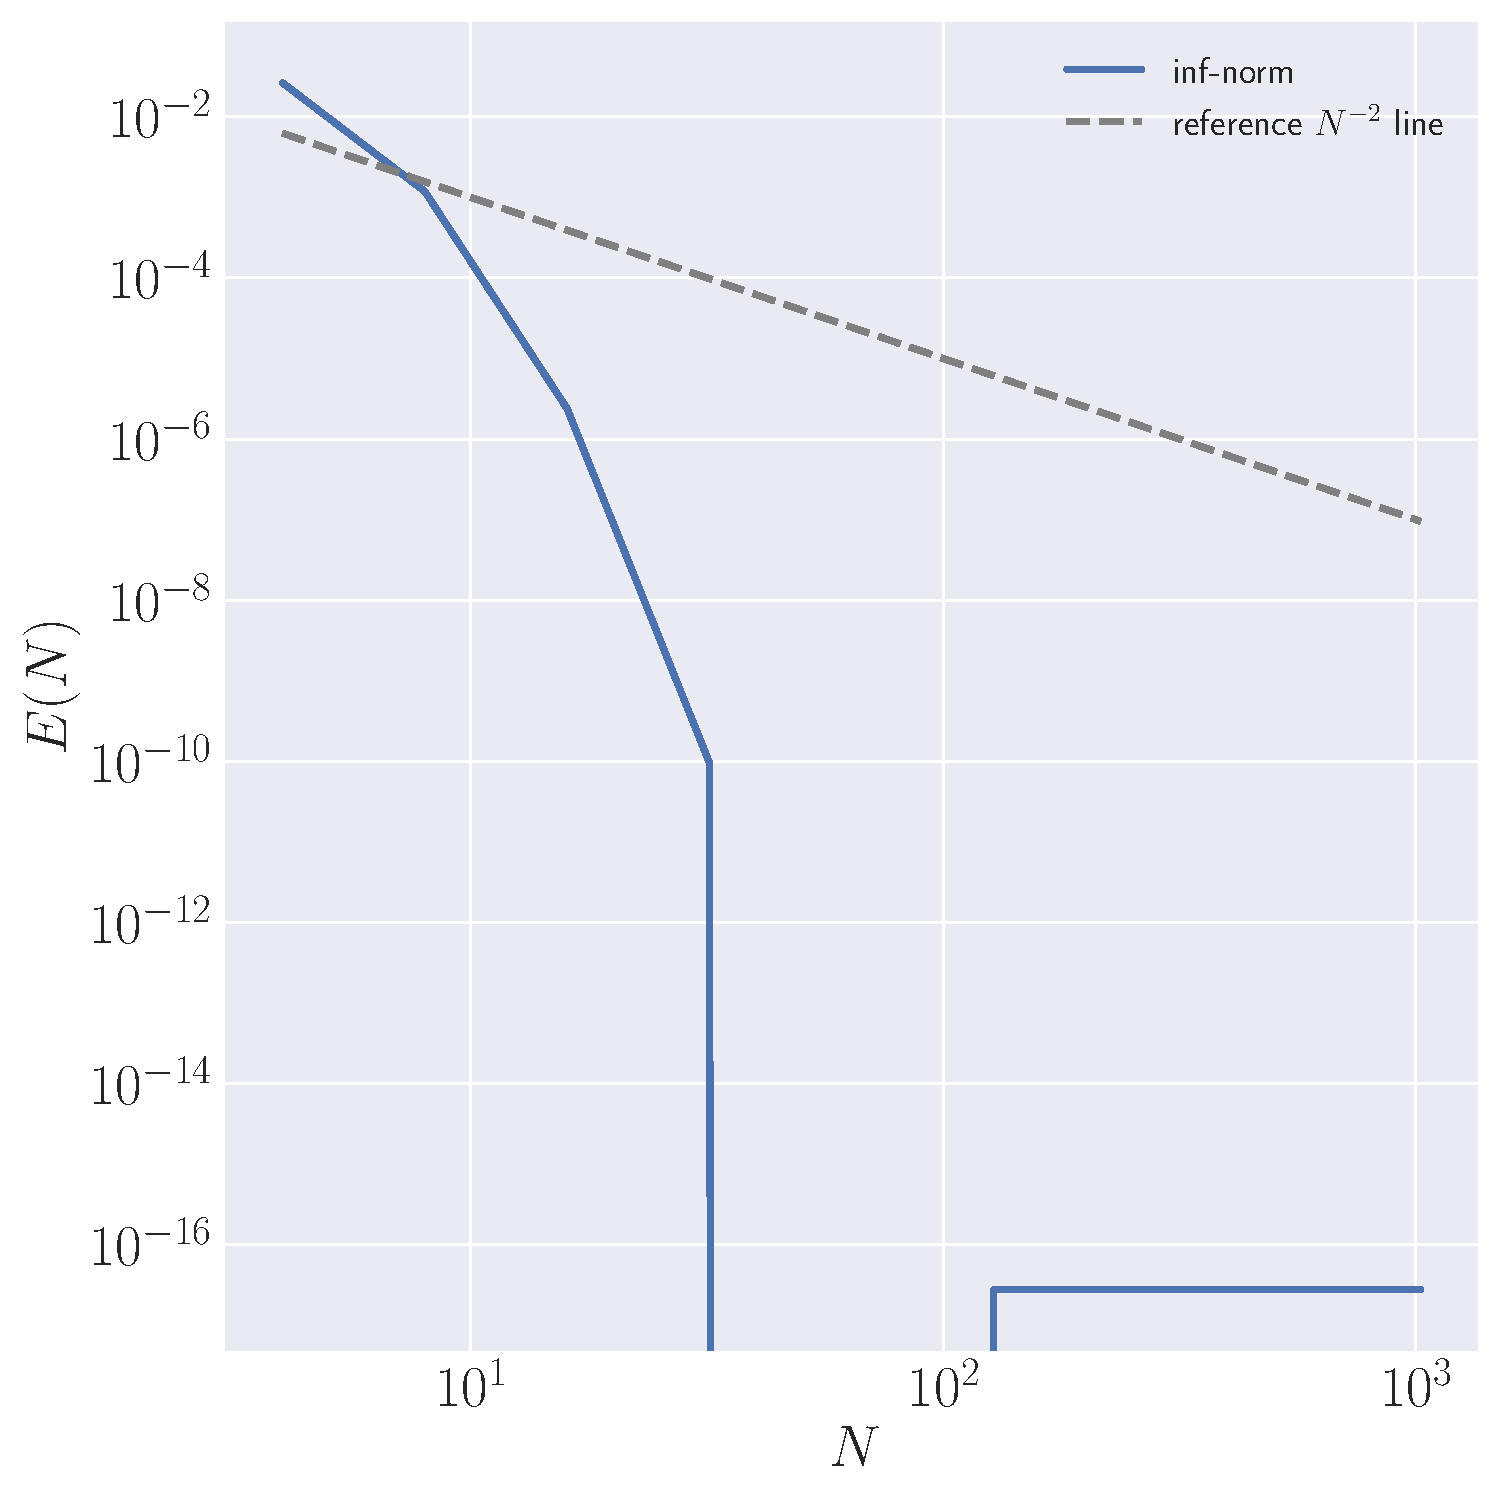
\includegraphics[clip, scale=0.3]{q1a_fig.pdf}
    \caption{Error of the solution of the differential equation $u^{\prime\prime} = 5\left(3+2\cos(\pi x)\right)^{-1}$ as a function of the number of intervals on the mesh.}
    \label{fig:q1a}
\end{figure}

\subsection*{Part B}

We observe from Fig.~\ref{fig:q1b} that this method, for the given RHS, is of order 1. The RHS function is continuous on the interval $[-1,1]$; however, its periodic extension across the real line is discontinuous at the edges. The first integral of the RHS function however is continuous on $[-1,1]$ and also has a continuous periodic extension on the real line. From this we infer that the function $u$ will also have continuous periodic extensions on the real line. From \textbf{[Tr]} we have, using Theorem 4 in Chapter 4, that 

\begin{theorem}
	If u has p-1 continuous derivatives in $L^{2}(\mathbb{R})$ for some $p\ge \nu + 1$, where $\nu$ denotes the $\nu$th spectral derivative of u on the grid $h\mathbb{Z}$, and a pth derivative of bounded variation, then $$|w_{j}-u^{(\nu)}(x_{j}) = \bO(h^{p-v})\quad \mathrm{as}\ h\to 0.$$
\end{theorem}

In this case we have $\nu = 1$ and $p=2$, and thus we expect an error scaling $\bO(h^{1})$, which agrees with our observation from Fig.~\ref{fig:q1b}.

\begin{figure}[!h]
    \centering
    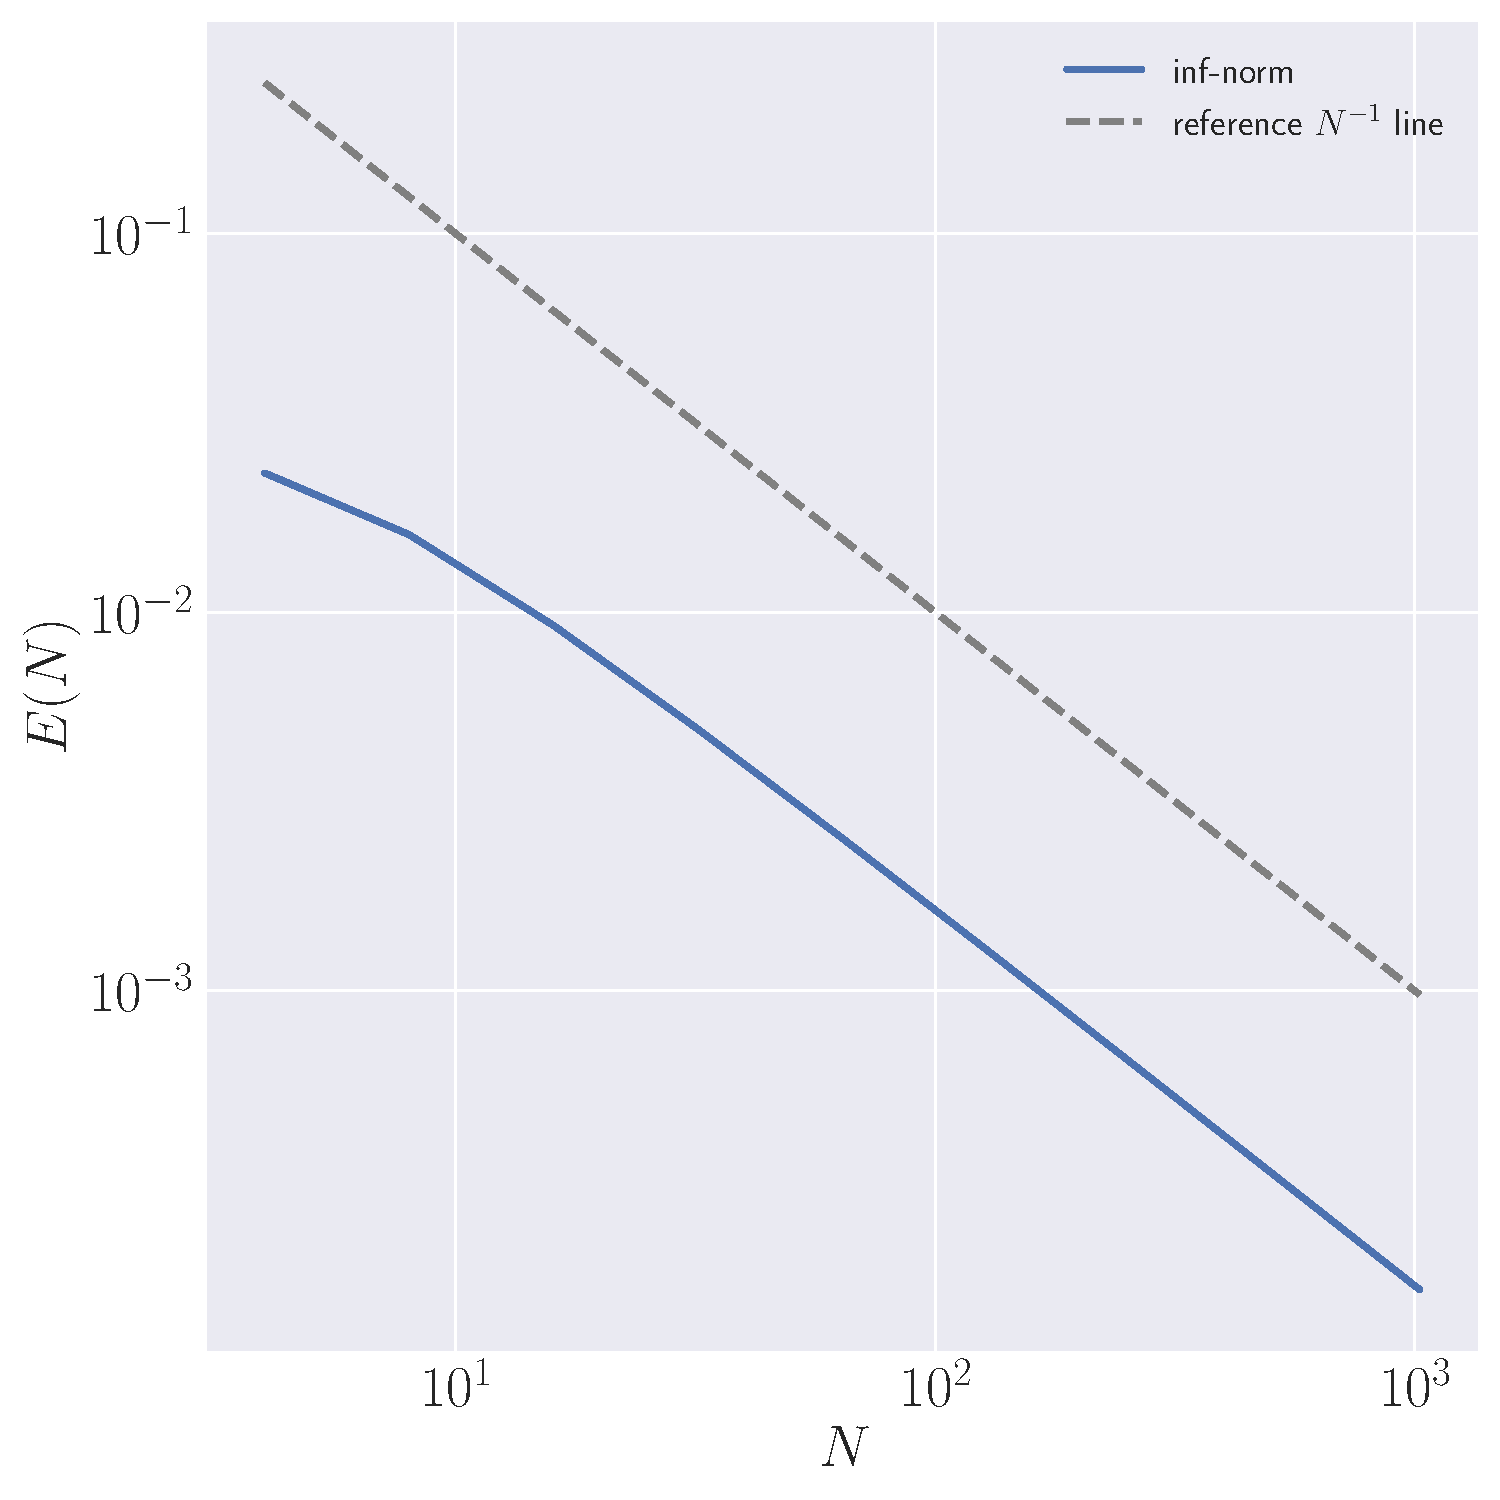
\includegraphics[clip, scale=0.3]{q1b_fig.pdf}
    \caption{Error of the solution of differential equation $u^{\prime\prime} = \sin(3\pi x/2)$ as a function of the number of intervals on the mesh.}
    \label{fig:q1b}
\end{figure}

\section*{Problem 2}

\subsection*{Part A}

The Discrete Fourier Transform is given by
\begin{align}
    u(x_{j}) = v_{j} &= \sum_{k=-\frac{N}{2}+1}^{\nicefrac{N}{2}} \vhat_{k}e^{ikx_{j}}.
\end{align}
The Fourier Expansion is given by
\begin{align}
    u(x_{j}) &= \sum_{k^{\prime}=-\infty}^{\infty} \hat{u}_{k^{\prime}}e^{ik^{\prime}x}
\end{align}
Writing the infinite sums as two sums, one over a finite range of wavenumbers $k$ and another over the range of wavenumbers $m$ not in that range (ie. write $k^{\prime} = k + mN$ ),
\begin{subequations}
    \begin{align}
        u(x_{j}) &= \sum_{k=-\frac{N}{2}+1}^{\nicefrac{N}{2}}\sum_{m=-\infty}^{\infty} \hat{u}_{k+mN}e^{i\left[k+mN\right]x_{j}}\\
        &= \sum_{k=-\frac{N}{2}+1}^{\nicefrac{N}{2}}\sum_{m=-\infty}^{\infty} \hat{u}_{k+mN}e^{ikx_{j}}e^{imNx_{j}}\\
        &= \sum_{k=-\frac{N}{2}+1}^{\nicefrac{N}{2}}\left[\sum_{m=-\infty}^{\infty} \hat{u}_{k+mN}\right]e^{ikx_{j}},
    \end{align}
\end{subequations} 
where we used that $e^{imNx_{j}} = e^{im\frac{2\pi}{h}jh} = e^{i(mj)2\pi} = 1\ \forall\ mj\in\mathbb{Z}$ in going from the penultimate to the last step. 
Thus equality between the Fourier Series Expansion and the Discrete Fourier Transform is held provided that 
\begin{align}
    \vhat_{k} = \sum_{m=-\infty}^{\infty} \hat{u}_{k+mN}.
\end{align}
Computing the aliasing error 
\begin{subequations}
    \begin{align}
        R_{N}u(x) &= I_{N}u(x) - T_{N}u(x)\\
        &= \sum_{k=-M}^{M}\vhat_{k}e^{ikx} - \sum_{k=-M}^{M}\hat{u}_{k}e^{ikx}\\
        &= \sum_{k=-M}^{M} \left[\vhat_{k}-\hat{u}_{k}\right]e^{ikx}\\
        &= \sum_{k=-M}^{M} \left[\left(\sum_{m=-\infty}^{\infty} \hat{u}_{k+mN}\right)-\hat{u}_{k}\right]e^{ikx}\\
        &= \sum_{k=-M}^{M} \left(\sum_{m=-\infty,m\neq 0}^{\infty} \hat{u}_{k+mN}\right)e^{ikx}.
    \end{align}
\end{subequations}
To show orthogonality of the aliasing and truncation errors, we compute their inner product
\begin{subequations}
	\begin{align}
		\hspace*{-1.5cm}\int_{0}^{2\pi}\dd{x}R_{N}u(x)\left[u(x)-T_{N}u(x)\right] &= \int_{0}^{2\pi}\dd{x}\left\{\sum_{k=-M}^{M} \left(\sum_{m=-\infty,m\neq 0}^{\infty} \hat{u}_{k+mN}\right)e^{ikx}\right\}\left\{u(x)-\sum_{k=-M}^{M}\hat{u}_{k}e^{ikx}\right\}\\
		&= \int_{0}^{2\pi}\dd{x}\left\{\sum_{k=-M}^{M} \left(\sum_{m=-\infty,m\neq 0}^{\infty} \hat{u}_{k+mN}\right)e^{ikx}\right\}\left\{\sum_{k=-\infty}^{\infty}\hat{u}_{k}e^{ikx}-\sum_{k=-M}^{M}\hat{u}_{k}e^{ikx}\right\}\\
		&= \int_{0}^{2\pi}\dd{x}\left\{\sum_{k=-M}^{M} \left(\sum_{m=-\infty,m\neq 0}^{\infty} \hat{u}_{k+mN}\right)e^{ikx}\right\}\left\{\sum_{k^{\prime}=-\infty}^{\infty}\hat{u}_{k^{\prime}}e^{ik^{\prime}x}\right\},
	\end{align}
\end{subequations}
where we have that $|k| < |k^{\prime}|$ (ie. the sum in the second $\{\cdot\}$ doesn't include any modes in the interval $|k| \le M$). Expanding gives,
\begin{subequations}
	\begin{align}
		&\int_{0}^{2\pi}\dd{x}\left\{\sum_{k=-M}^{M} \left(\sum_{m=-\infty,m\neq 0}^{\infty} \hat{u}_{k+mN}\right)e^{ikx}\right\}\left\{\sum_{k^{\prime}=-\infty}^{\infty}\hat{u}_{k^{\prime}}e^{ik^{\prime}x}\right\}\\
		&= \int_{0}^{2\pi}\dd{x}\left\{\sum_{k=-M}^{M}\sum_{k^{\prime}=-\infty}^{\infty}\sum_{m=-\infty,m\neq 0}^{\infty} \hat{u}_{k+mN}\hat{u}_{k^{\prime}}e^{i(k+k^{\prime})x}\right\}\\
		&= \sum_{k=-M}^{M}\sum_{k^{\prime}=-\infty}^{\infty}\sum_{m=-\infty,m\neq 0}^{\infty} \int_{0}^{2\pi}\dd{x}\hat{u}_{k+mN}\hat{u}_{k^{\prime}}e^{i(k+k^{\prime})x}.
	\end{align}
\end{subequations}
The integral will be nonzero in value only when $k=-k^{\prime}$ by orthogonality of complex exponentials; however, this will never be satisfied as the domain of $k$ is disjoint from the domain of $k^{\prime}$ and therefore the integral is always zero. Thus, we have that 
\begin{align}
	\int_{0}^{2\pi}\dd{x}R_{N}u(x)\left[u(x)-T_{N}u(x)\right] = 0
\end{align}
and thereby the two errors are orthogonal. Now if we take the equality
\begin{align}
	u(x) - I_{N}u(x) = (u(x)-T_{N}u(x)) - R_{N}u(x),
\end{align}
square both sides,
\begin{subequations}
	\begin{align}
		\left[u(x) - I_{N}u(x)\right]^{2} &= \left[(u(x)-T_{N}u(x)) - R_{N}u(x)\right]^{2}\\
		u(x)^{2} - 2\left[I_{N}u(x)\right]u(x) + \left[I_{N}u(x)\right]^{2} &= 
		(u(x)-T_{N}u(x))^{2} - 2(u(x)-T_{N}u(x))R_{N}u(x) + \left[R_{N}u(x)\right]^{2},\\
	\end{align}
\end{subequations}
and then integrate on the domain,
\begin{subequations}
	\begin{align}
		\hspace*{-1.5cm}\int_{0}^{2\pi}\dd{x}\left[u(x) - I_{N}u(x)\right]^{2} &= \int_{0}^{2\pi}\dd{x}(u(x)-T_{N}u(x))^{2} - 2\int_{0}^{2\pi}\dd{x}(u(x)-T_{N}u(x))R_{N}u(x) + \int_{0}^{2\pi}\dd{x}\left[R_{N}u(x)\right]^{2}\\
		\left||u(x) - I_{N}u(x)\right||^{2} &= \left||u(x)-T_{N}u(x)\right||^{2} + \left||R_{N}u(x)\right||^{2},
	\end{align}
\end{subequations}
where the cross-term on the right-hand side vanishes via the orthogonality.


\subsection*{Part B}

We see in Fig.~\ref{fig:q2b_interpolant_plot}, for the first and second functions ($u_{1}(x)$ and $u_{2}(x)$, respectively) that the interpolant is behaving as expected. It is going through the grid points; however, for lower values of $N$ it tends to not be a very good approximation for the function. For the last function $u_{3}$ we observe that the interpolant is very badly behaved. This behaviour is arising due to aliasing of the underlying function. The underlying function is sinusoidal with wavenumber $k=32$. Thus, in order to represent this using its Fourier series, the series must contain at least this mode and all others beneath it.  

\begin{figure}[!h]
    \centering
    \subfloat{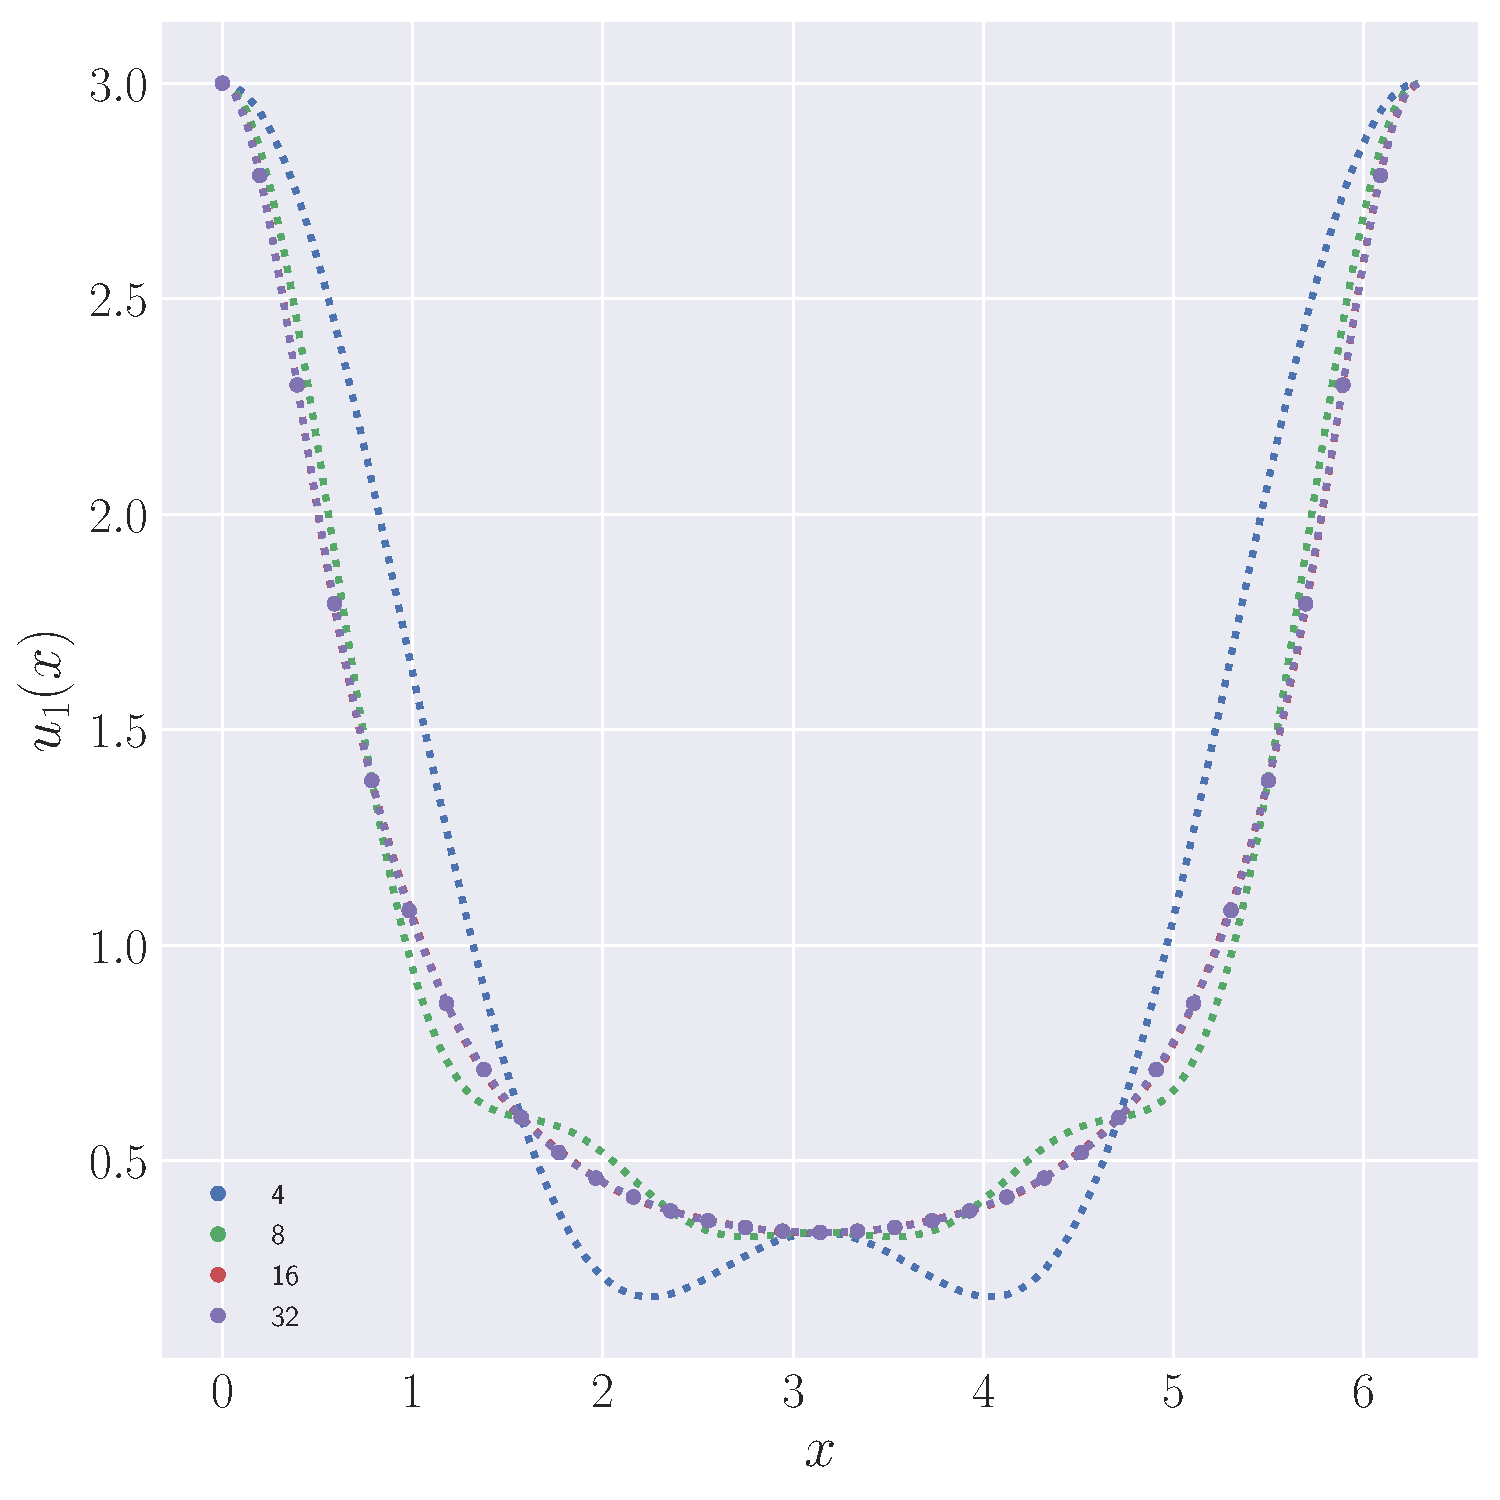
\includegraphics[clip, scale=0.2]{q2b_func1_interpolant_figure.pdf}}
    \subfloat{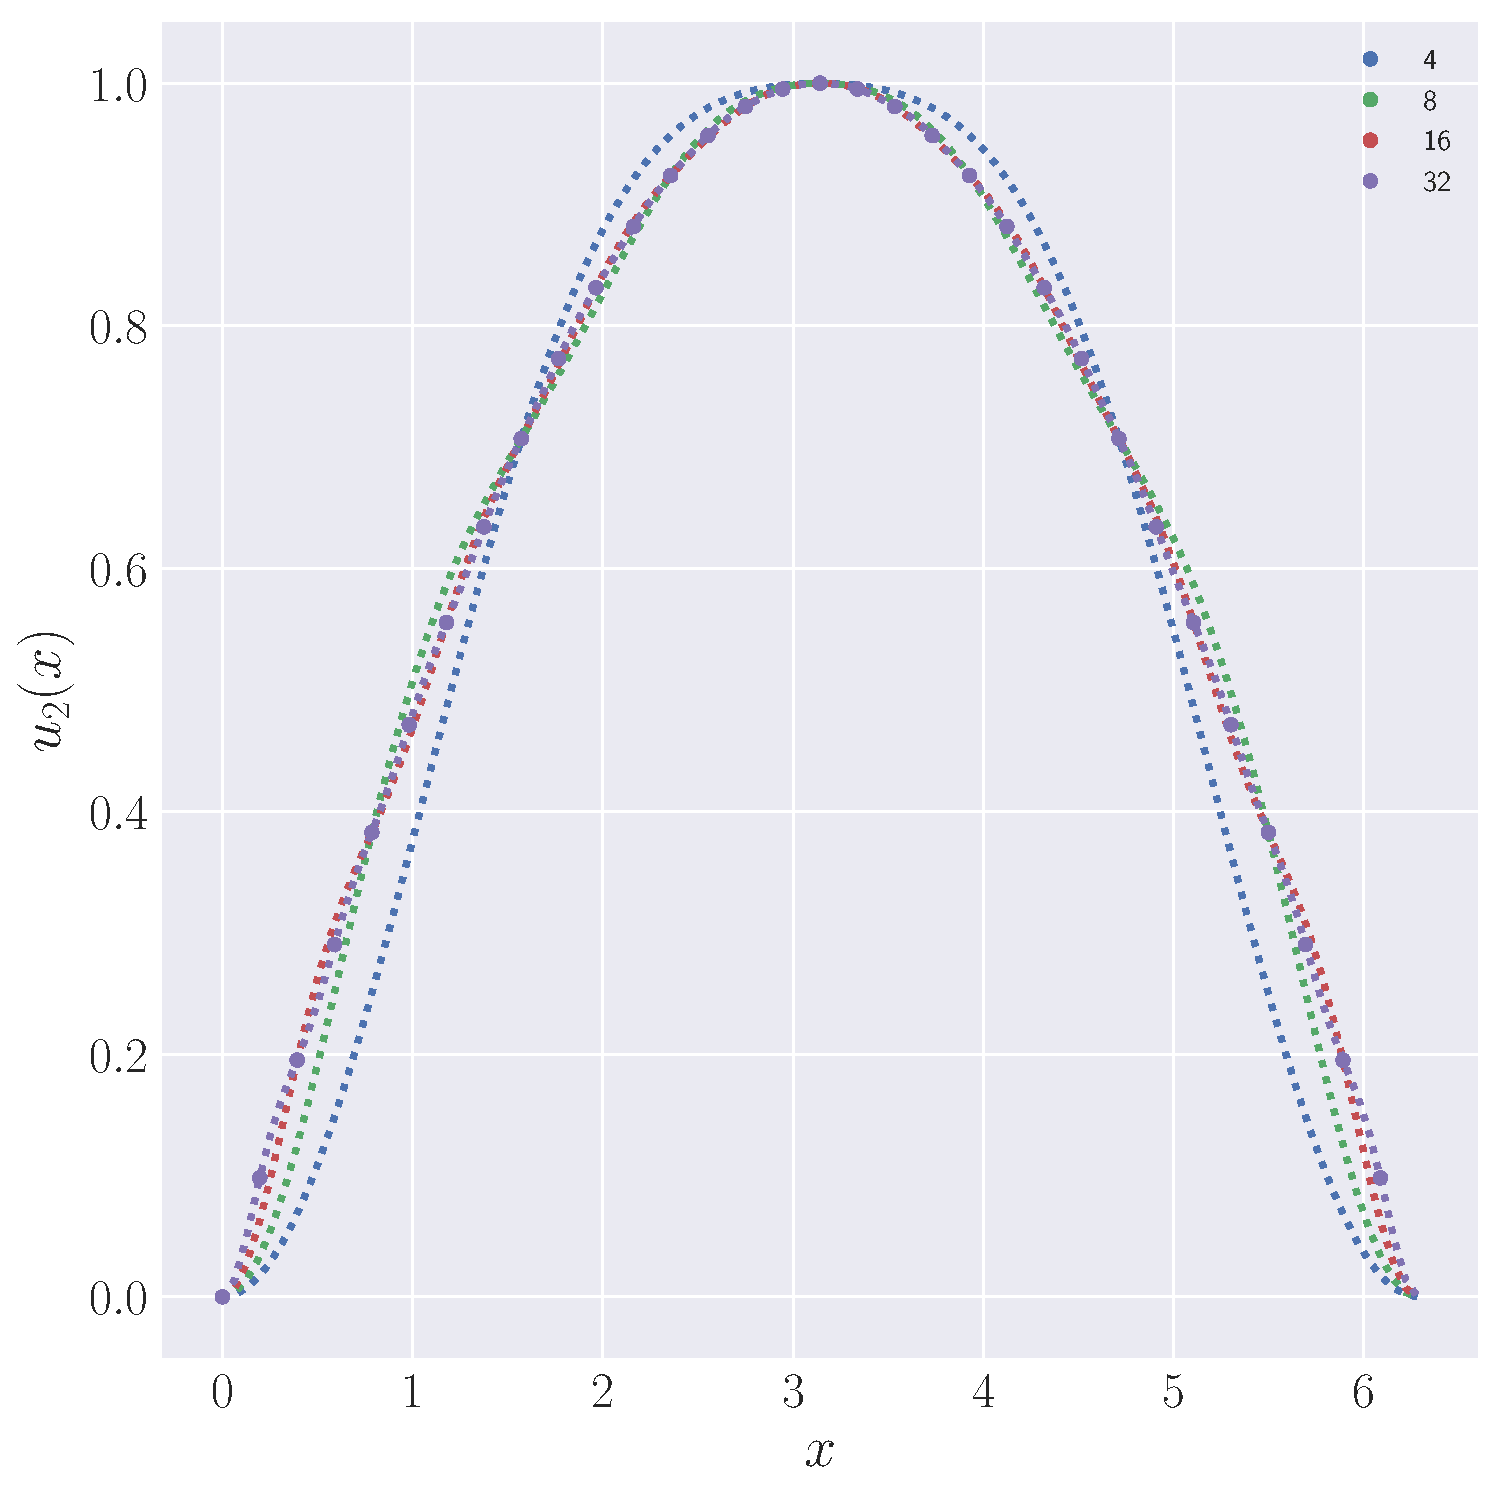
\includegraphics[clip, scale=0.2]{q2b_func2_interpolant_figure.pdf}}
    \subfloat{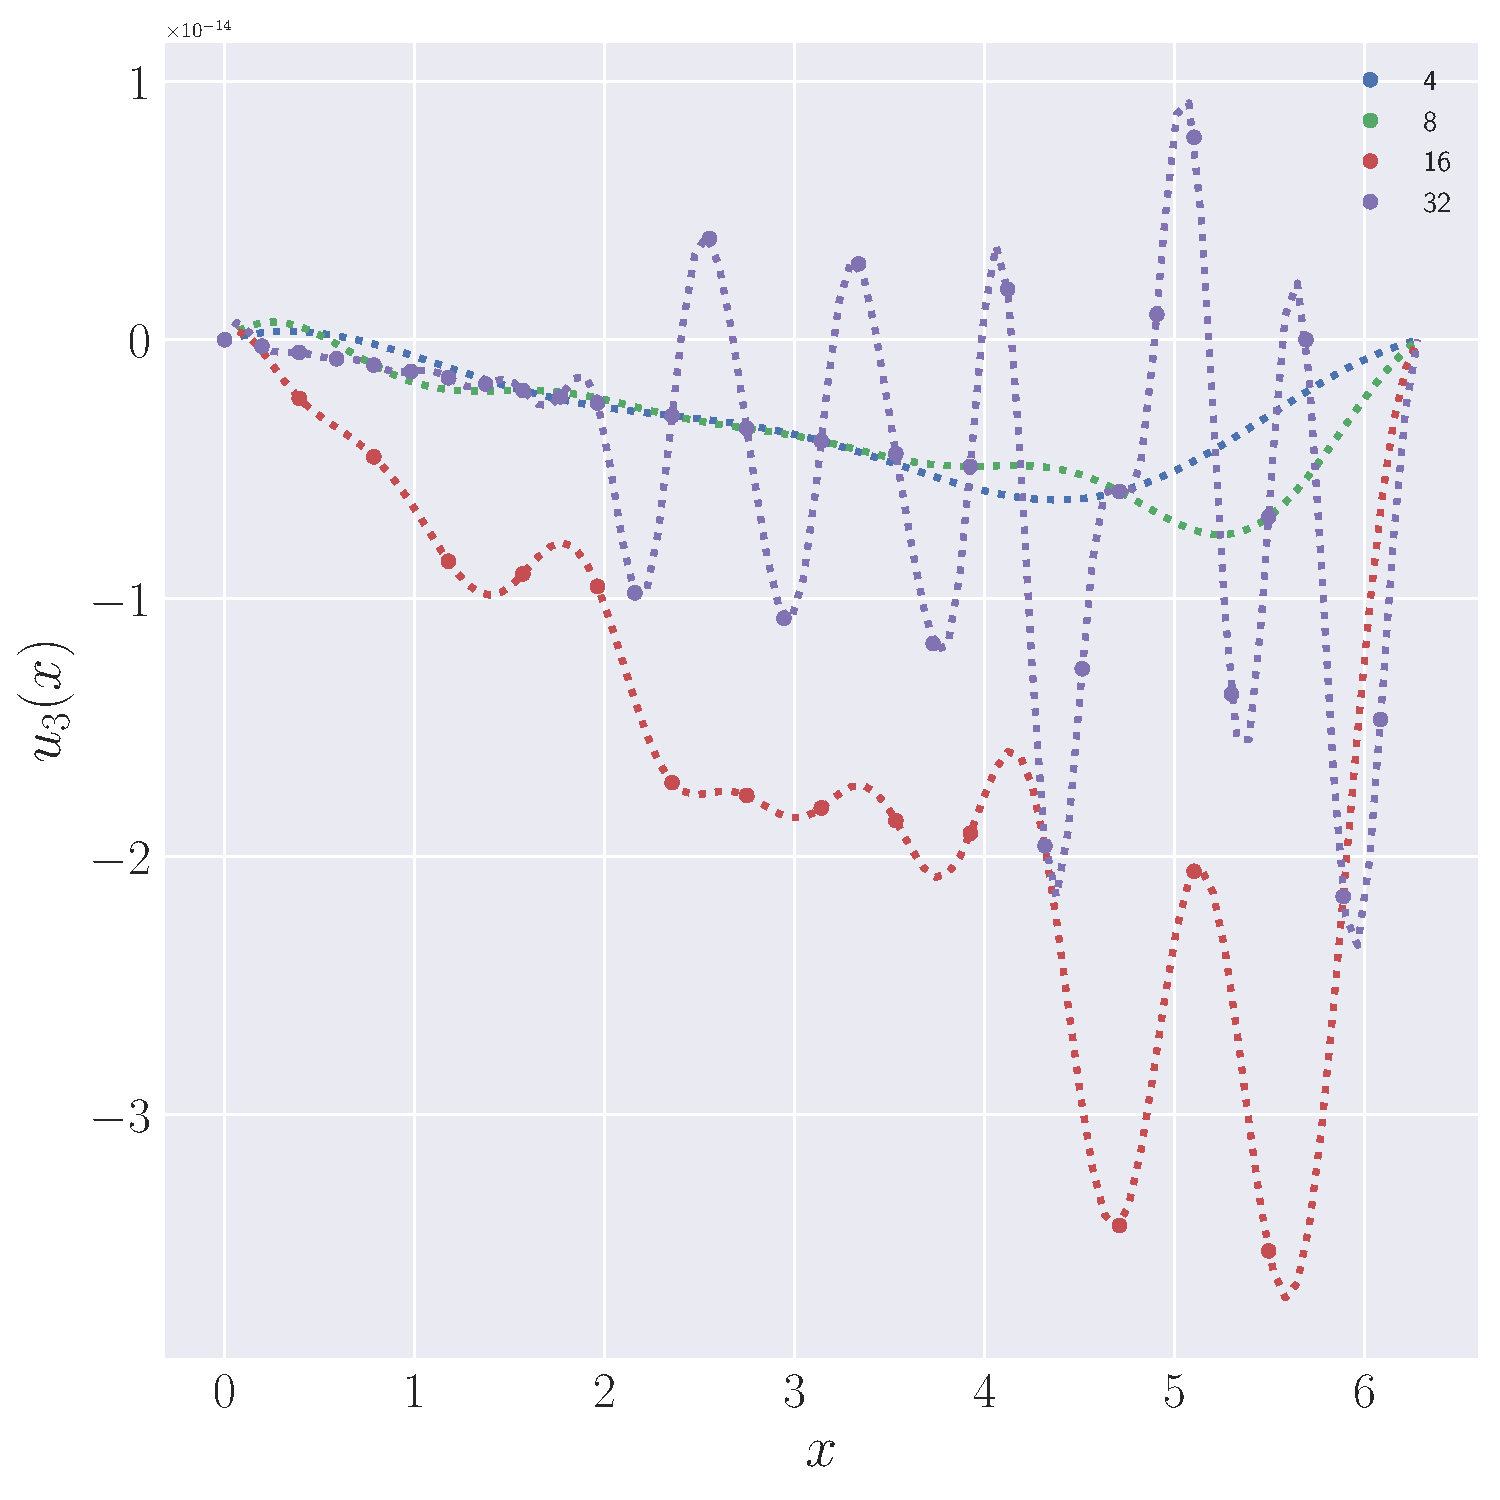
\includegraphics[clip, scale=0.2]{q2b_func3_interpolant_figure.pdf}}
    \caption{
        Interpolant calculated for the function $u_{1}(x) = 3\left(5-4\cos x\right)^{-1}$ [left subplot], $u_{2}(x) = \sin(x/2)$ [middle subplot],  $u_{3}(x) = \sin(32x)$ [right subplot] for number of grid points $N = 4, 8, 16, 32$. Data markers indicate the function evaluated on the grid points. Dotted lines denote the interpolant evaluated on a grid of 100 points.
    }
    \label{fig:q2b_interpolant_plot}
\end{figure}

From Fig.~\ref{fig:q2b_interpolant_truncation_plot}, we observe that for the functions $u_{1}(x)$ and $u_{2}(x)$ that while the interpolant is directly equivalent to the function $u$ on the grid, the truncated Fourier series doesn't interpolate those points exactly.  

In \verb|A3Q2.ipynb| I show that $\vhat_{k} \neq \hat{u}_{k}$ for the first case of $u_{1}(x)$; however, I am unable to show numerically the folding of the frequencies outside the Nyquist bandwidth.

\begin{figure}[!h]
    \centering
    \subfloat{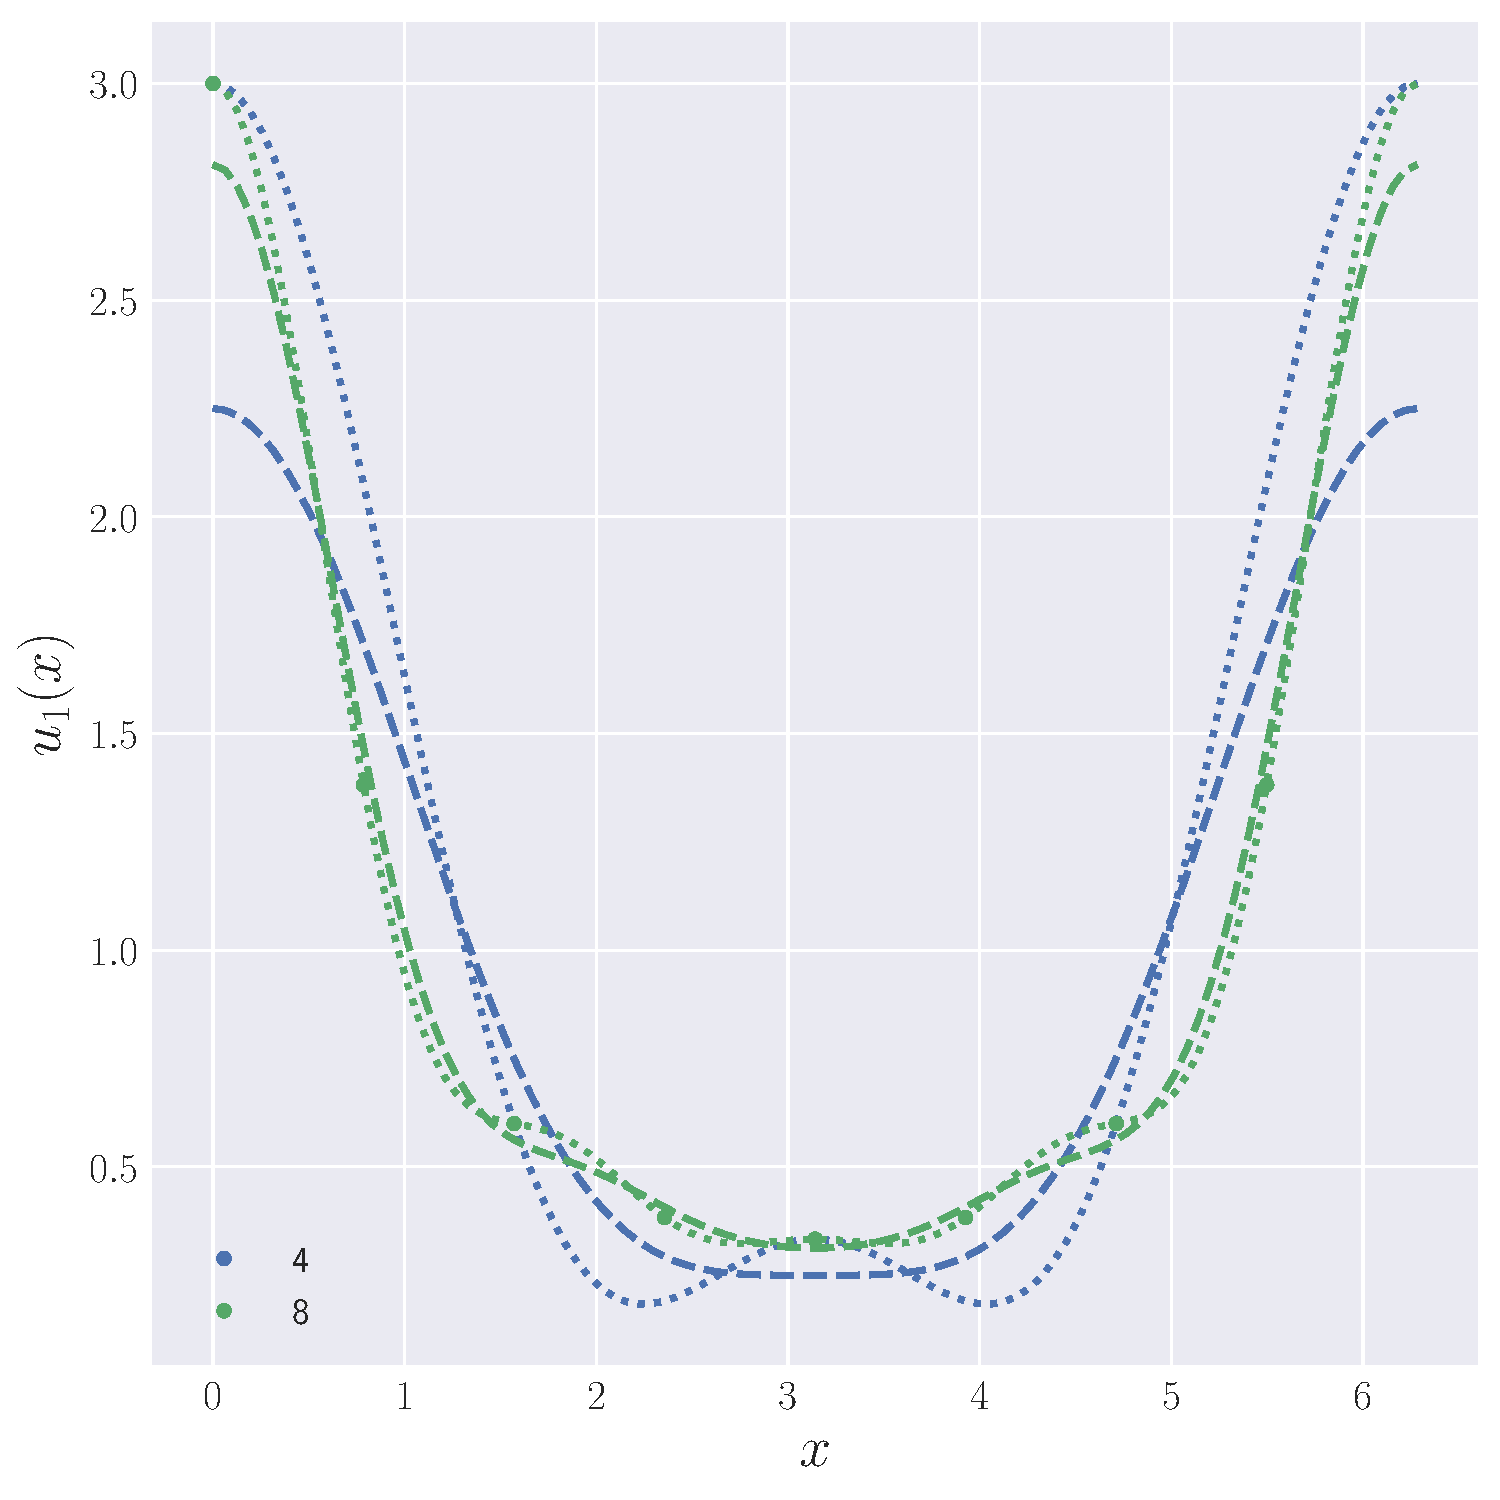
\includegraphics[clip, scale=0.2]{q2b_func1_interpolant_truncation_figure.pdf}}
    \subfloat{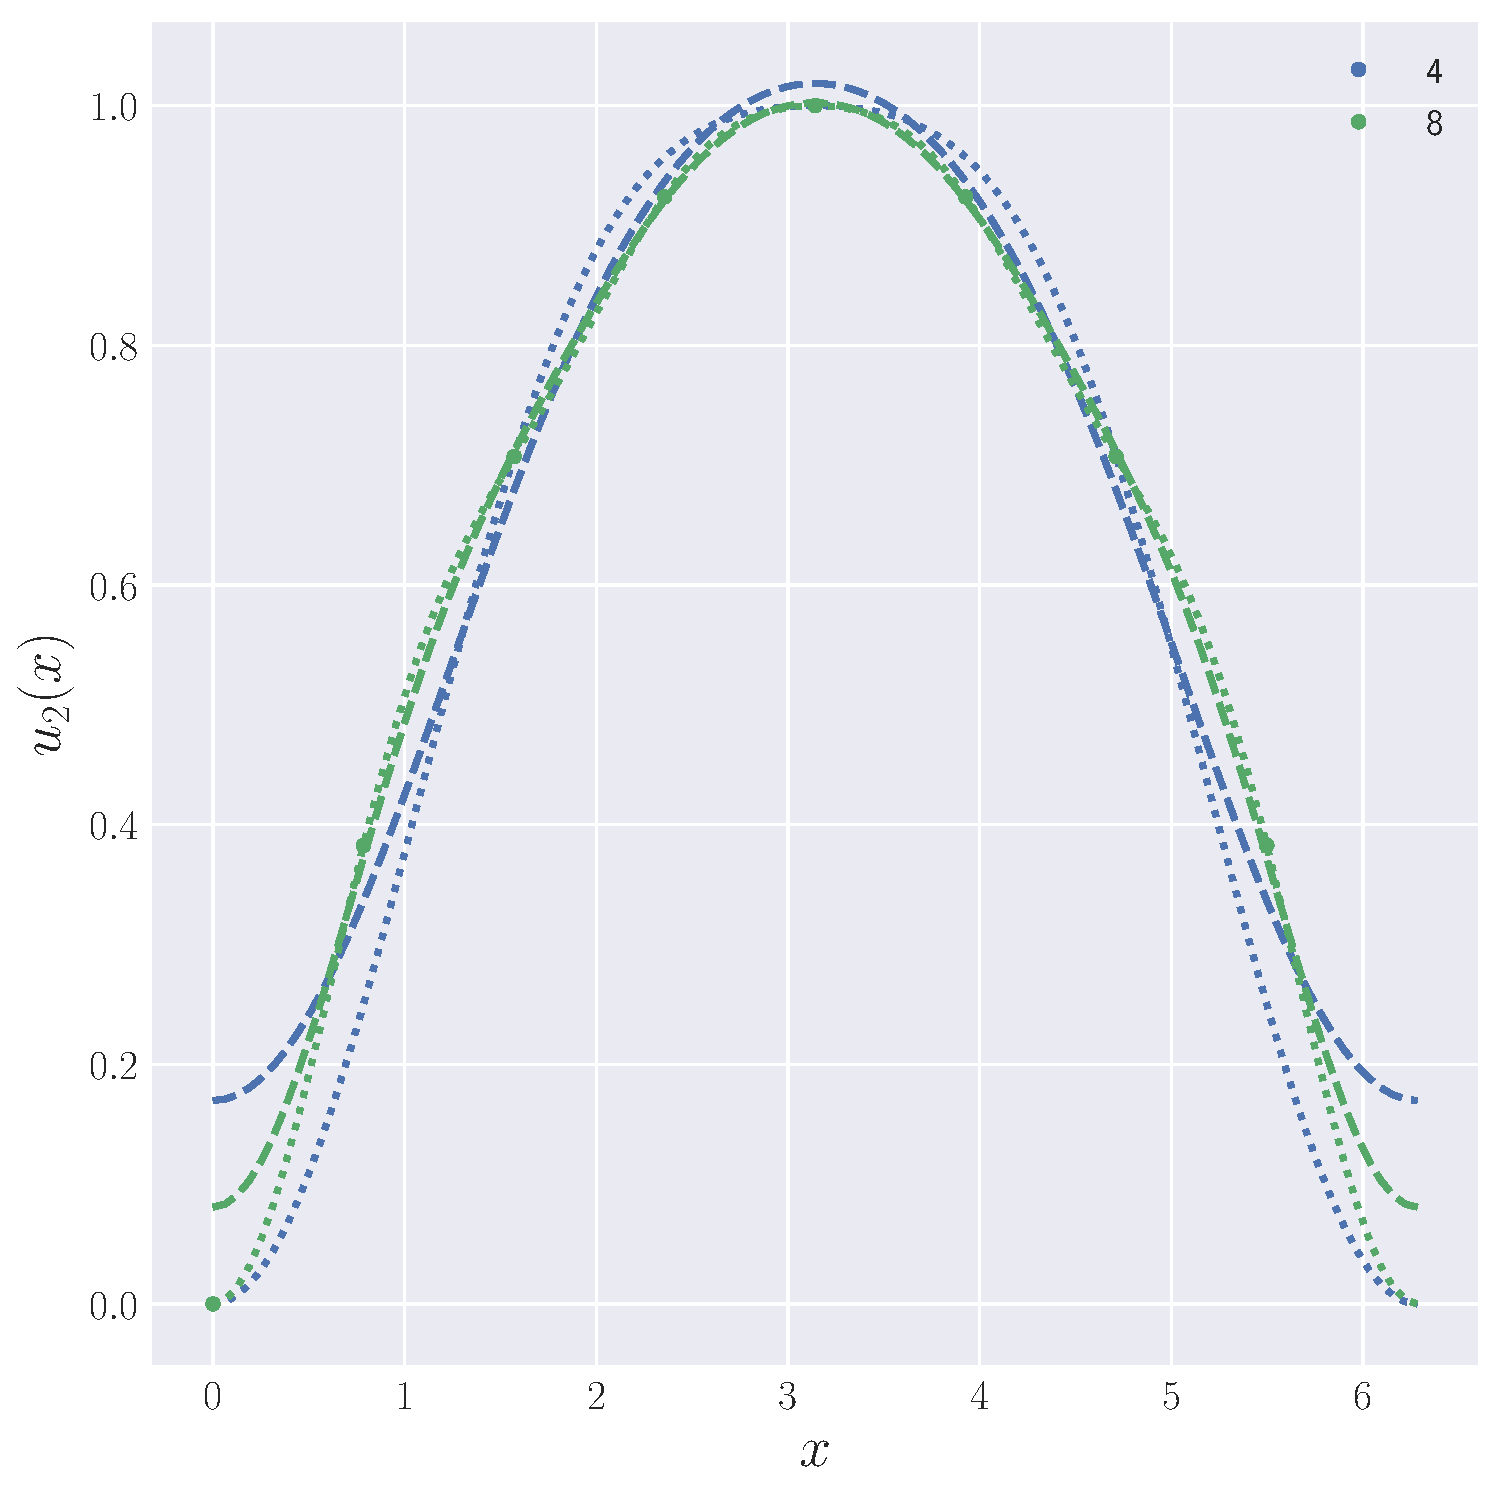
\includegraphics[clip, scale=0.2]{q2b_func2_interpolant_truncation_figure.pdf}}
    \subfloat{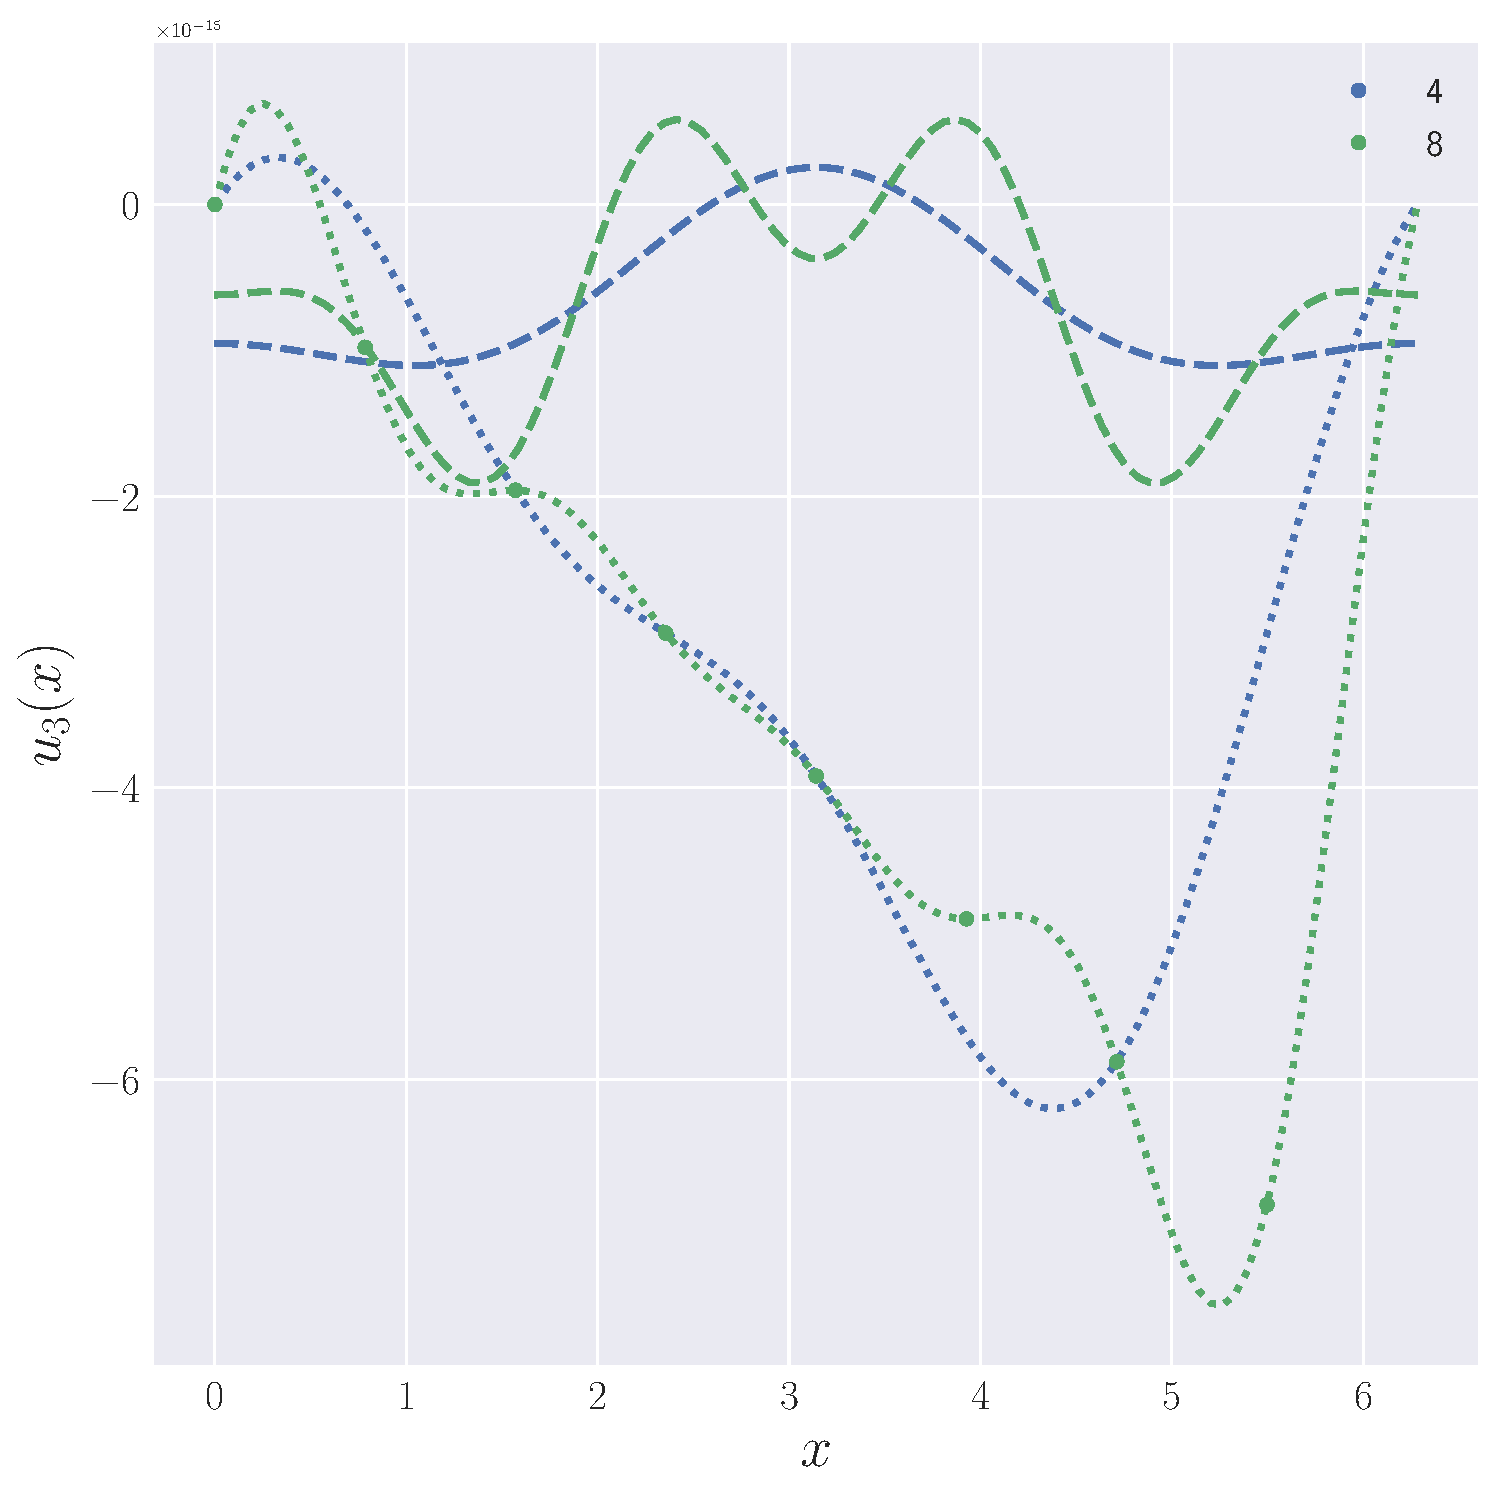
\includegraphics[clip, scale=0.2]{q2b_func3_interpolant_truncation_figure.pdf}}
    \caption{
        Interpolant and truncated Fourier Series calculated for the functions functions $u_{1}(x) = 3\left(5-4\cos x\right)^{-1}$ [left subplot], 
        $u_{2}(x) = \sin(x/2)$ [middle subplot], $u_{3}(x) = \sin(32x)$ [right subplot] for number of grid points $N = 4, 8$. 
        Data markers indicate the function evaluated on the grid points. 
        Dotted lines denote the interpolant. 
        Dashed lines denote the truncated Fourier Series. 
        Different colors denote different number of \emph{grid} points.  
        Both interpolant and truncated Fourier Series are evaluated on a finer grid of 100 points.
    }
    \label{fig:q2b_interpolant_truncation_plot}
\end{figure}

In Fig.~\ref{fig:q2b_interpolant_truncation_error_plot} we see the interpolation error (blue lines) and the truncation error (green lines) for the functions $u_{1}(x)$, $u_{2}(x)$, and $u_{3}(x)$. In the left subplot we observe that for $u_{1}(x)$ the error in both the interpolation and truncation decrease at the same rate initially; however, at $N > 100$ the interpolation error remains low while the truncation error increases drastically. This is a manifestation of spectral blocking where noise accumulates heavily in the largest wavenumbers. In the middle subplot, for $u_{2}(x)$ we observe that the error scaling is polynomial (the behaviour does change at larger $N$). This is due to the fact that the function's periodic extension is discontinuous and thus we expect that the error would not have spectral convergence. In the right subplot, for $u_{3}(x)$ we see that the interpolation and the truncation error stay constant for until $N > 64$ when the Nyquist criterion becomes fulfilled and the interpolation error decreases significantly; however, the truncation error stays constant.

\begin{figure}[!h]
    \centering
    \subfloat{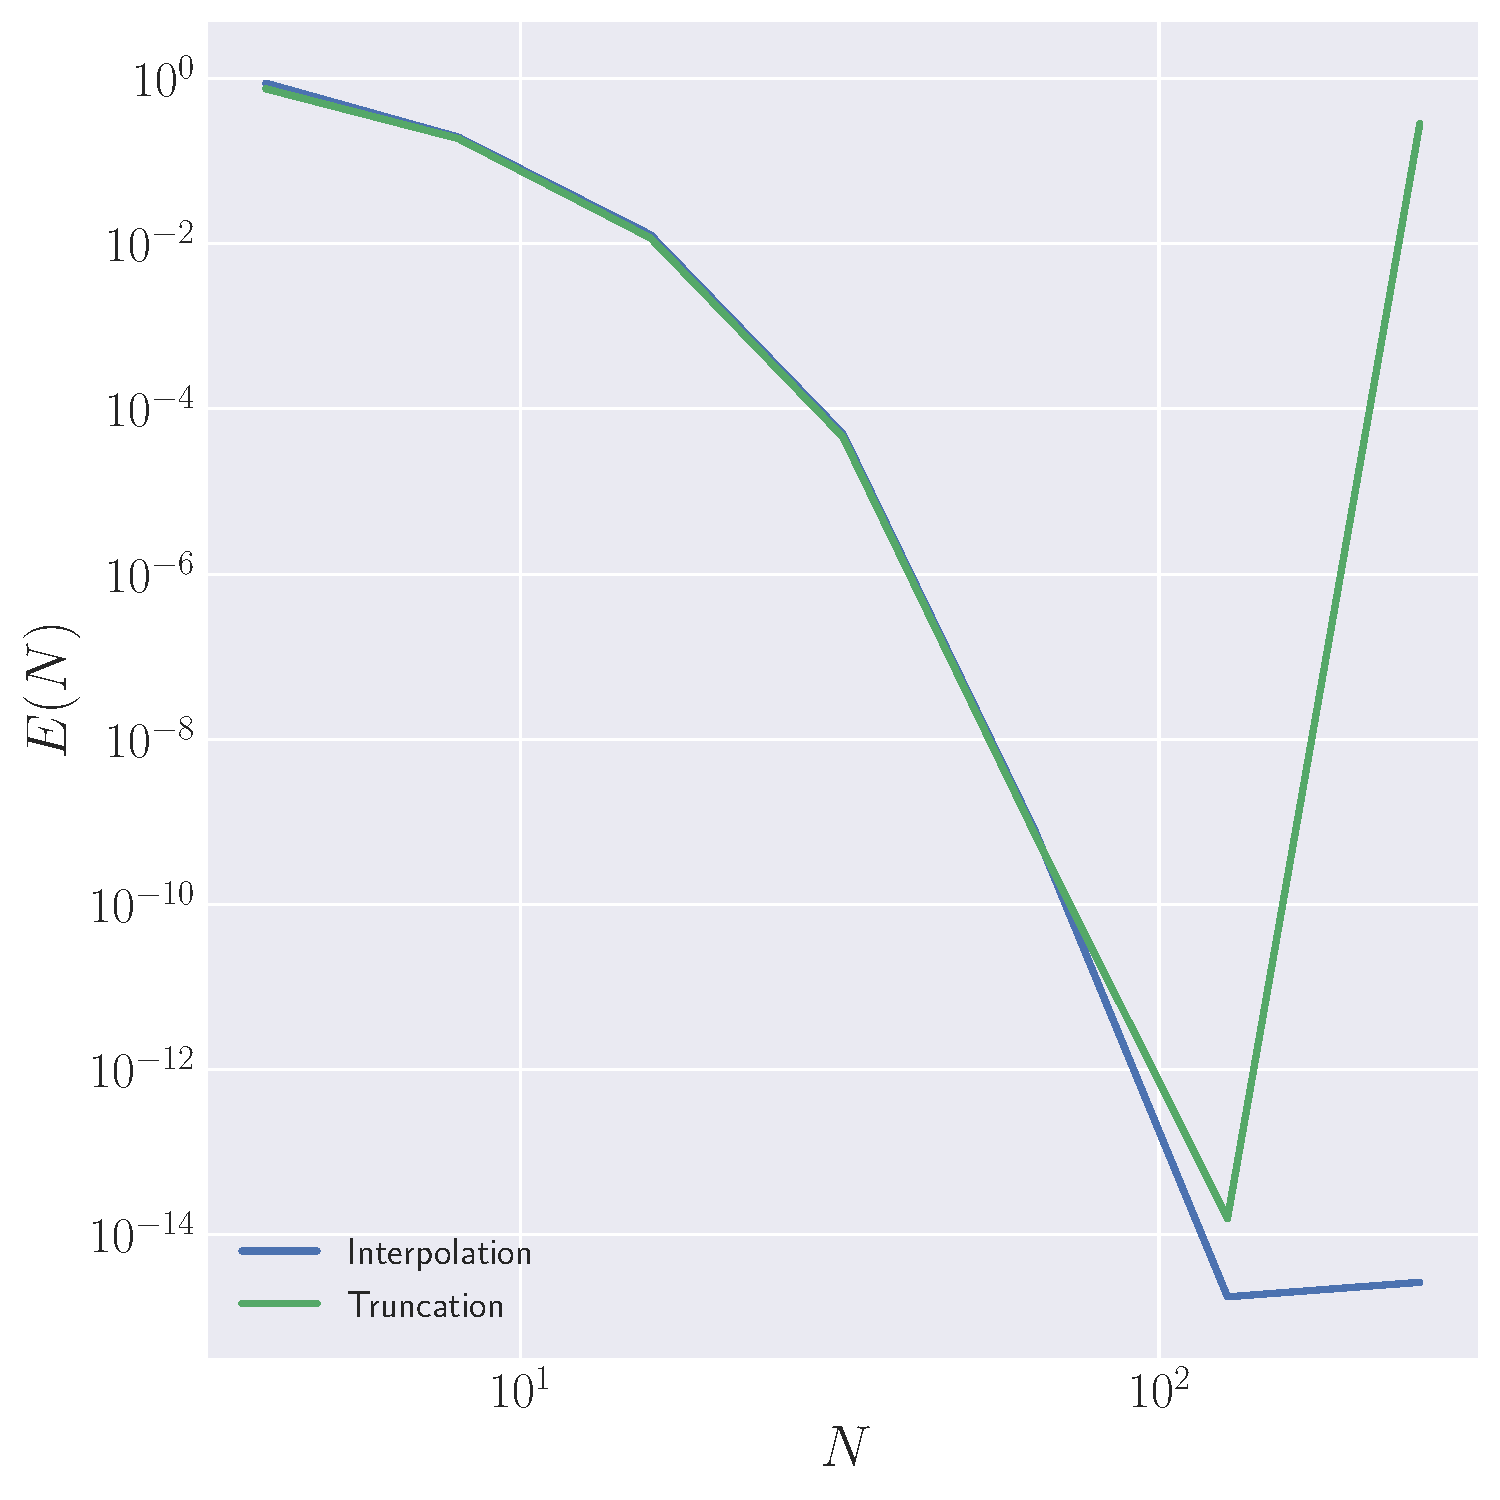
\includegraphics[clip, scale=0.2]{q2b_func1_trunc_interp_error_fig.pdf}}
    \subfloat{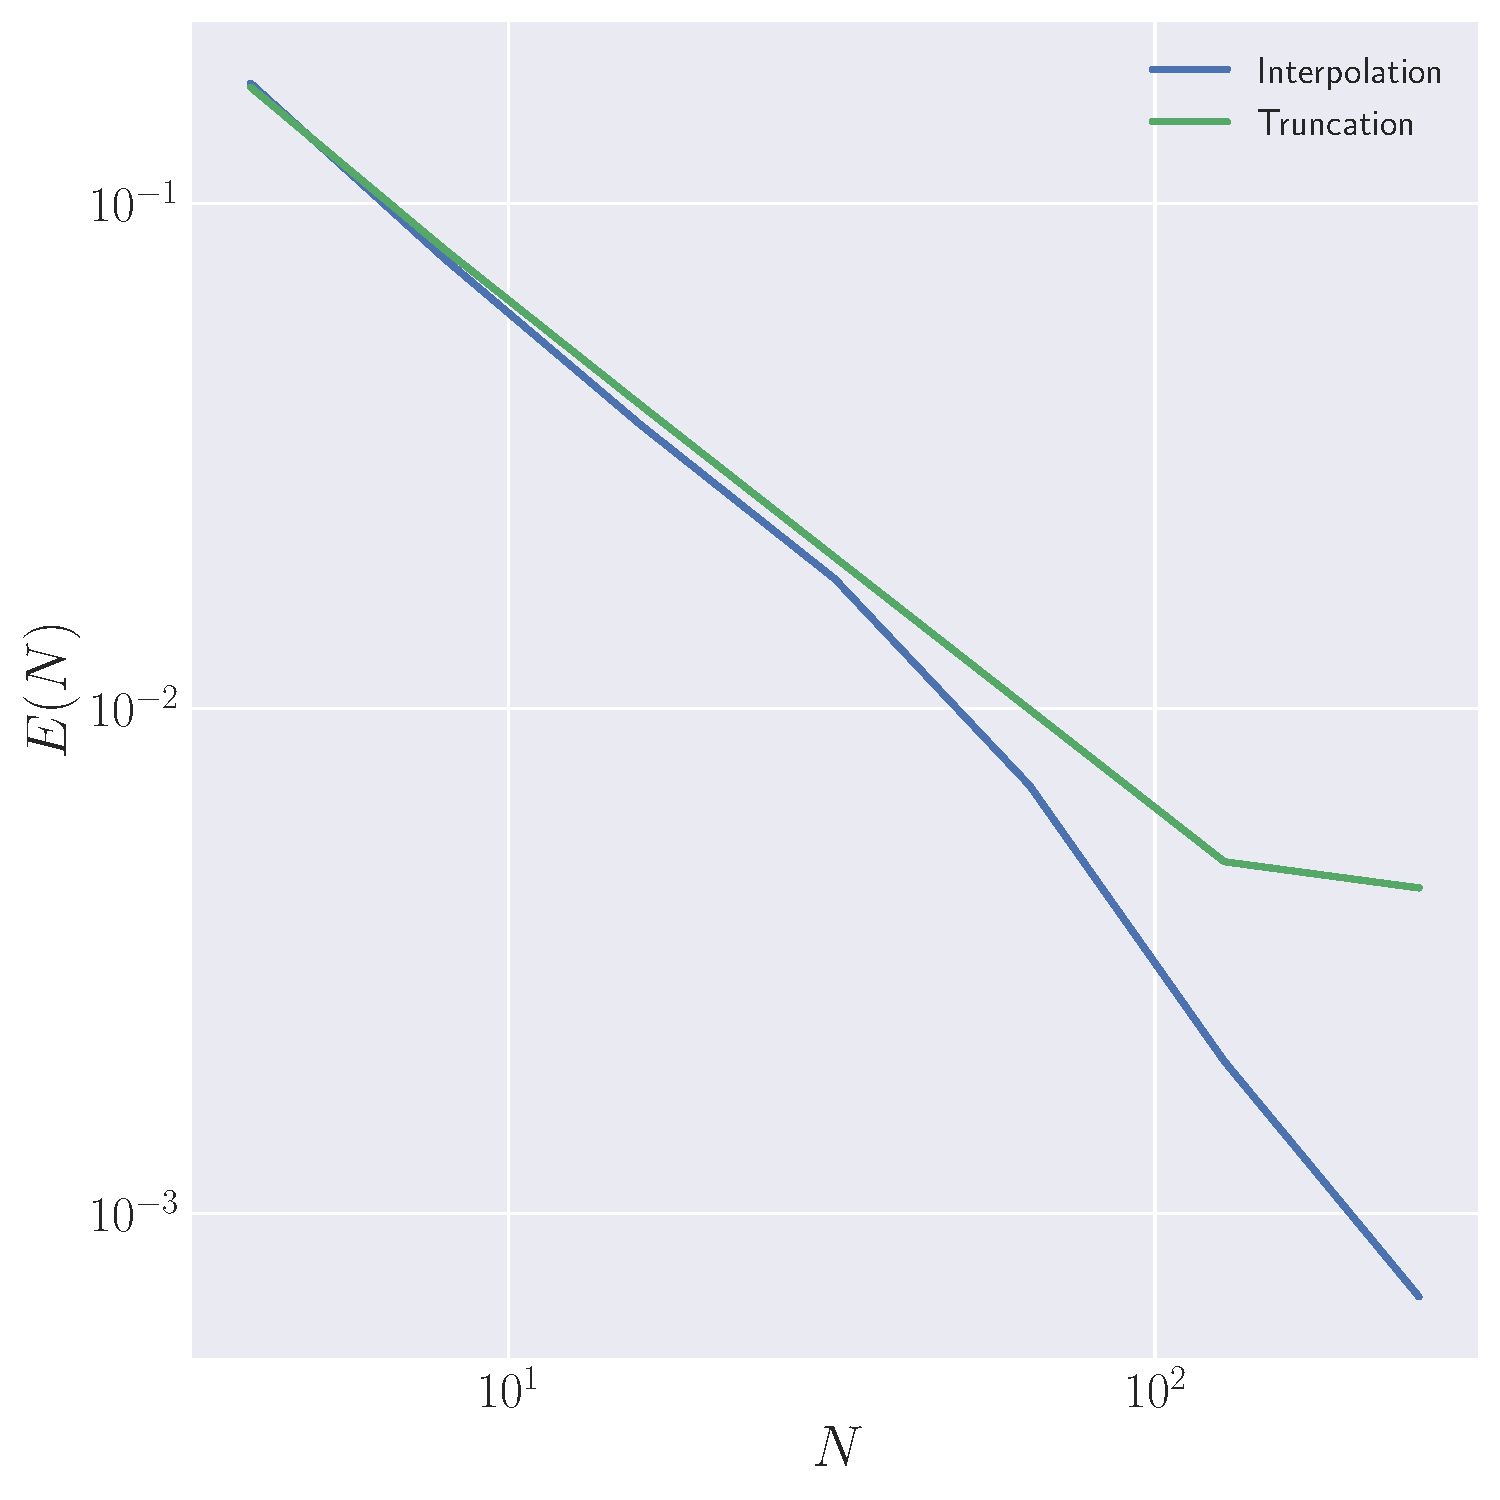
\includegraphics[clip, scale=0.2]{q2b_func2_trunc_interp_error_fig.pdf}}
    \subfloat{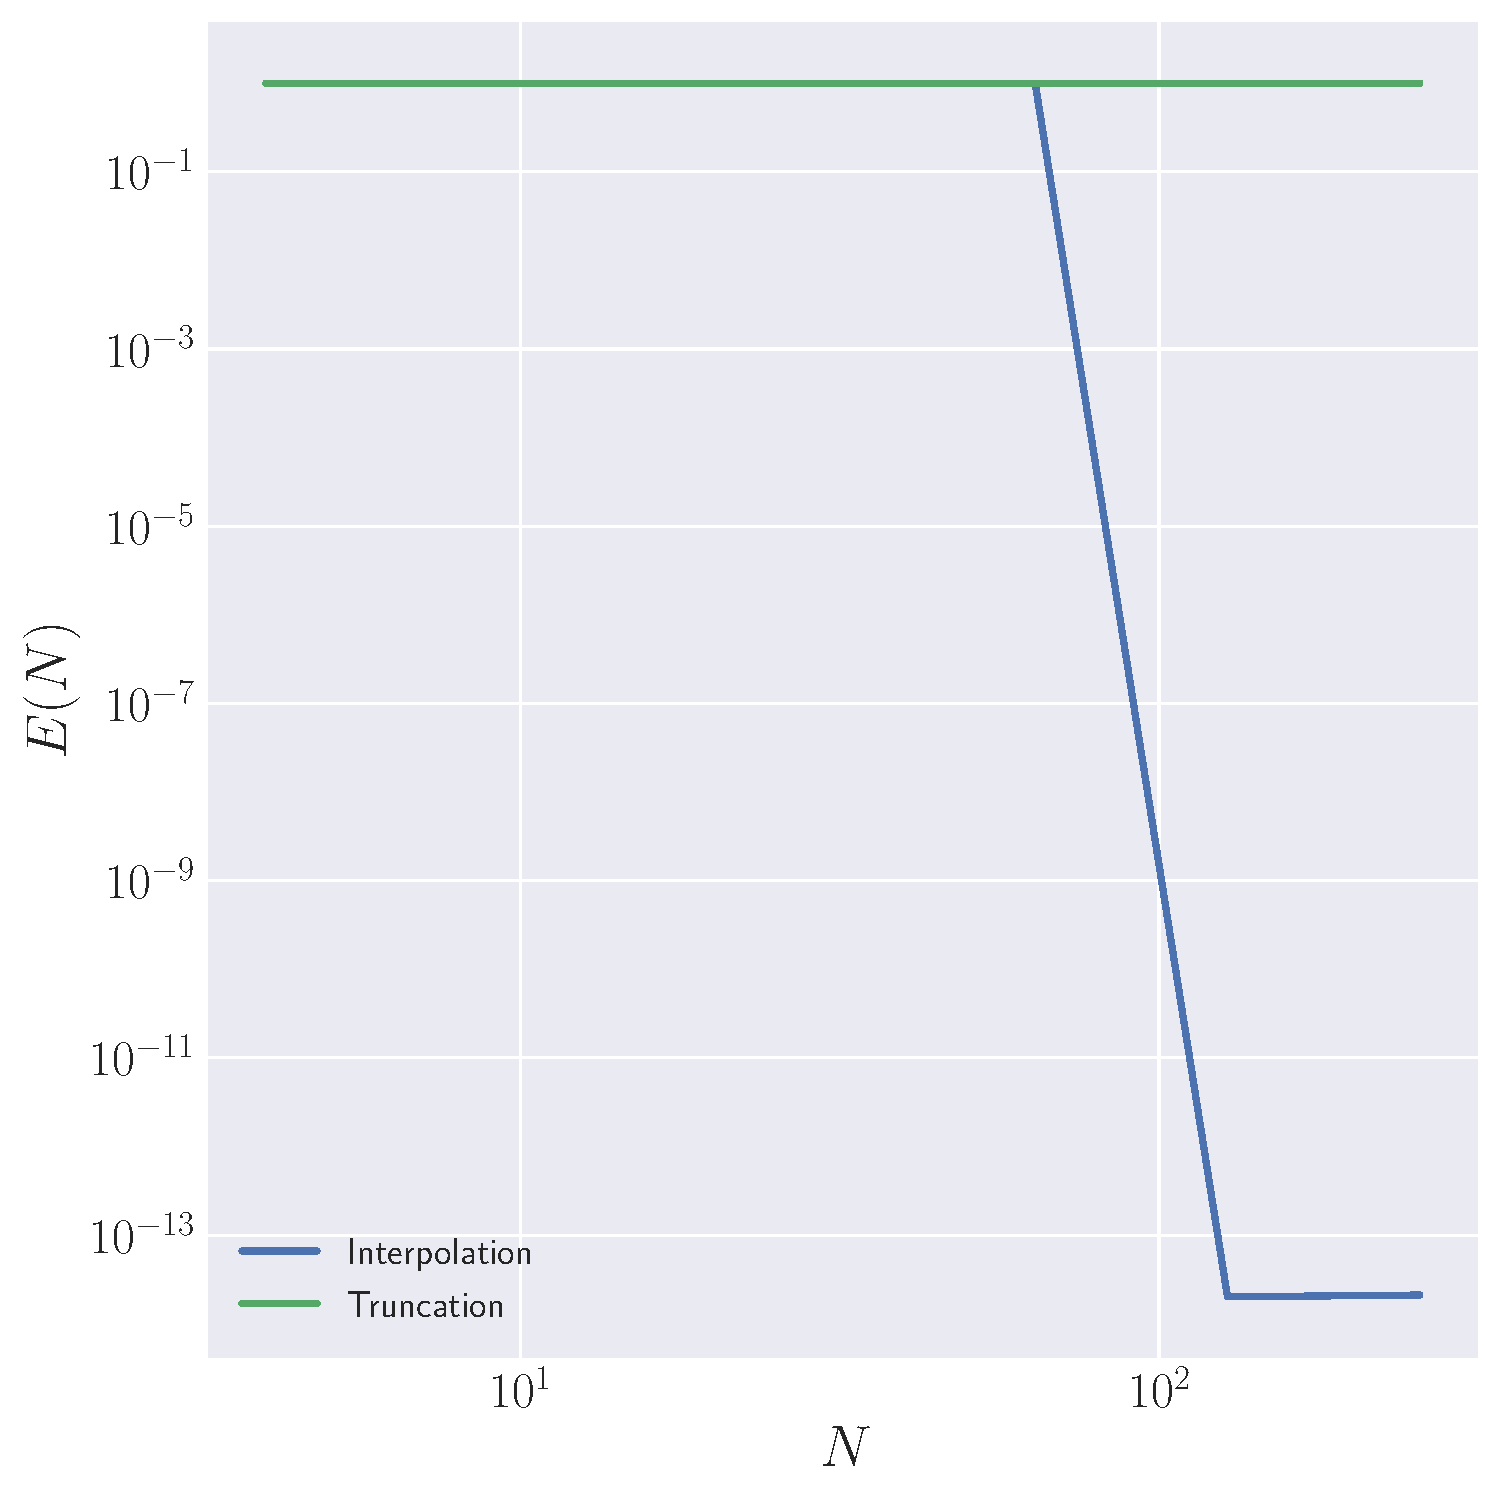
\includegraphics[clip, scale=0.2]{q2b_func3_trunc_interp_error_fig.pdf}}
    \caption{
        Error of the interpolation (blue line) and truncated Fourier Series (green line) calculated for the functions $u_{1}(x) = 3\left(5-4\cos x\right)^{-1}$ [left subplot], 
        $u_{2}(x) = \sin(x/2)$ [middle subplot], $u_{3}(x) = \sin(32x)$ [right subplot]. 
    }
    \label{fig:q2b_interpolant_truncation_error_plot}
\end{figure}

\section*{Problem 3}

\subsection*{Part A}

Taking the logarithm of the Lagrange Polynomial we get
\begin{subequations}
    \begin{align}
        \log(L_{j}(x)) &= \log\left[\dfrac{\prod_{k=0,k\neq j}^{N}(x-x_{k})}{\prod_{k=0,k\neq j}^{N}(x_{j}-x_{k})}\right]\\
        & = \log\left[\prod_{k=0,k\neq j}^{N}\dfrac{(x-x_{k})}{(x_{j}-x_{k})}\right]\\
        &= \sum_{k=0,k\neq j}^{N} \log\left(\dfrac{x-x_{k}}{x_{j}-x_{k}}\right).
    \end{align}
\end{subequations}
Now taking derivatives,
\begin{subequations}
    \begin{align}
        \dfrac{1}{L_{j}(x)}L_{j}^{\prime}(x) &= \sum_{k=0,k\neq j}^{N}\dfrac{x_{j}-x_{k}}{x-x_{k}}\left[\dfrac{1}{x_{j}-x_{k}}\right]\\
        \implies L_{j}^{\prime}(x) &= L_{j}(x) \sum_{k=0,k\neq j}^{N}\dfrac{1}{x-x_{k}}.
    \end{align}
\end{subequations}
Evaluating at points $x_{i}$ to acquire the definitions for the entries of the differentiation matrix $D$. When $i\neq j$ we have
\begin{subequations}
    \begin{align}
        D_{ij} = L_{j}^{\prime}(x_{i}) &= L_{j}(x_{i}) \sum_{k=0,k\neq j}^{N}\dfrac{1}{x_{i}-x_{k}}\\
        &= \left[\prod_{k=0,k\neq j}^{N}\dfrac{(x_{i}-x_{k})}{(x_{j}-x_{k})}\right]\sum_{k=0,k\neq j}^{N}\dfrac{1}{x_{i}-x_{k}}\\
        &= \left[\prod_{k=0,k\neq j}^{N}\dfrac{1}{(x_{j}-x_{k})}\right]\sum_{k=0,k\neq j}^{N}\left[\prod_{k=0,k\neq j}^{N}(x_{i}-x_{k})\right]\dfrac{1}{x_{i}-x_{k}}\\
        &= \dfrac{1}{a_{j}}\prod_{k=0,k\neq i,j}^{N}(x_{i}-x_{k})\\
        &= \dfrac{1}{a_{j}}\prod_{k=0,k\neq i}^{N}\dfrac{(x_{i}-x_{k})}{(x_{i}-x_{j})}\\
        &= \dfrac{1}{a_{j}}\dfrac{\prod_{k=0,k\neq i}^{N}(x_{i}-x_{k})}{(x_{i}-x_{j})}\\
        &= \dfrac{1}{a_{j}}\dfrac{a_{i}}{(x_{i}-x_{j})}
    \end{align}
\end{subequations}
When $i=j$ we have
\begin{subequations}
    \begin{align}
        D_{ii} = L_{i}(x_{i}) &= L_{i}(x_{i}) \sum_{k=0,k\neq j}^{N}\dfrac{1}{x_{i}-x_{k}}\\
        &= \left[\prod_{k=0,k\neq j}^{N}\dfrac{(x_{i}-x_{k})}{(x_{i}-x_{k})}\right]\sum_{k=0,k\neq j}^{N}\dfrac{1}{x_{i}-x_{k}}\\
        &= \sum_{k=0,k\neq j}^{N}\dfrac{1}{x_{i}-x_{k}}
    \end{align}
\end{subequations}
Taking a summation over the rows gives
\begin{subequations}
    \begin{align}
        \sum\limits_{j=0, j\neq i}^{N} D_{ij} &= \sum\limits_{j=0, j\neq i}^{N}\dfrac{1}{a_{j}}\dfrac{a_{i}}{(x_{i}-x_{j})}\\
        &= a_{i}\sum\limits_{j=0, j\neq i}^{N}\left[\prod_{k=0,k\neq j}^{N}\dfrac{1}{(x_{j}-x_{k})}\right]\dfrac{1}{(x_{i}-x_{j})}
    \end{align}
\end{subequations}

Finding the interpolant to the vector of ones, $\vb{a}$,
\begin{subequations}
    \begin{align}
        p(x) &= \sum_{j=0}^{N} L_{j}(x)a_{j}\\
        &= \sum_{j=0}^{N} L_{j}(x).
    \end{align}
\end{subequations}
Evaluating at any given grid point $x_{i}$, gives 
\begin{subequations}
    \begin{align}
        p(x_{i}) &= \sum_{j=0}^{N} L_{j}(x_{i})\\
        &= \sum_{j=0}^{N} \delta_{ij}\\
        &= 1.
    \end{align}
\end{subequations}
This has to be the case, as if the matrix $D$ is associated with differentiation, then a differentiation of a constant function must be zero.
Since any constant function, evaluated on a grid, can be represented by $f(x_{i}) = c\vb{a}$ then it follows that for $D$ to be an approximation to a differentiation matrix, that $D\vb{a} = \vb{0}$.

\subsection*{Part C}

For the $N = 5$ the spectral radius is calculated to be $\approx 0$ modulo roundoff error; however, for $N=20$ the spectral radius of the Chebyshev matrix is $\approx 3.38$. Since the spectral radius provides a lower bound on the magnitude of the 2-norm, then this shows that the Chebyshev matrix will never achieve a matrix-2norm value of less than $3.38$ and therefore, will not satisfy $D_{20}^{21} = 0$. 
This arises from the fact that the matrix is poorly-conditioned.

\end{document}